% !TeX root = Laporan.tex
% Laporan Tugas Besar Data Mining: Conference Popularity and Association Pattern Mining (DBLP)
% Kompilasi: ./build.sh  (xelatex -> biber -> xelatex x2)
\documentclass[oneside]{kp-sti}

\addbibresource{daftar-pustaka.bib}

% --- Tambahan preamble: warna, pustaka TikZ, dan gaya diagram ---
\usepackage{rotating}
\usetikzlibrary{patterns,decorations.pathreplacing}
\definecolor{bluemain}{HTML}{2A78D6}
\definecolor{bluelight}{HTML}{9EC5F4}
\definecolor{orangemain}{HTML}{EB6834}
\definecolor{graymid}{HTML}{B9B8B2}
\definecolor{grayline}{HTML}{E3E3DF}
\definecolor{hx104281}{HTML}{104281}
\definecolor{hx1C5CAB}{HTML}{1C5CAB}
\definecolor{hx2A78D6}{HTML}{2A78D6}
\definecolor{hx3987E5}{HTML}{3987E5}
\definecolor{hx5598E7}{HTML}{5598E7}
\definecolor{hx6DA7EC}{HTML}{6DA7EC}
\definecolor{hx86B6EF}{HTML}{86B6EF}
\definecolor{hx9EC5F4}{HTML}{9EC5F4}
\definecolor{hxCDE2FB}{HTML}{CDE2FB}
% Tanda kutip judul pada daftar pustaka (glyph kutip bawaan tidak tampil pada font ini)
\DeclareFieldFormat[article,inproceedings,incollection]{title}{\char"201C #1\char"201D}
\setlength{\cftfignumwidth}{3.4em}\setlength{\cfttabnumwidth}{3.4em}
\renewcommand{\topfraction}{0.9}\renewcommand{\bottomfraction}{0.8}\renewcommand{\textfraction}{0.08}\renewcommand{\floatpagefraction}{0.75}
\makeatletter\setlength{\@fptop}{0pt}\setlength{\@fpsep}{10pt plus 1fil}\setlength{\@fpbot}{0pt plus 2fil}\makeatother
\titlespacing*{\section}{0pt}{14pt}{6pt}\titlespacing*{\subsection}{0pt}{10pt}{6pt}
\newsavebox{\kotakfig}
\newlength{\figmaxh}\setlength{\figmaxh}{8.4cm}
\newcommand{\figtikz}[2][\figmaxh]{%
  \sbox{\kotakfig}{\input{images/#2}}%
  \pgfmathsetmacro{\figscale}{min(1,\linewidth/\wd\kotakfig,#1/\ht\kotakfig)}%
  \scalebox{\figscale}{\usebox{\kotakfig}}}
\tikzset{
  proses/.style={kotak,fill=bluelight!35,draw=bluemain},
  berkas/.style={kotak,fill=grayline!60,draw=black!60,rounded corners=4pt},
  rencana/.style={kotak,dashed,draw=black!50,fill=white},
  abu/.style={kotak,fill=grayline,draw=graymid},
  buang/.style={kotak,fill=orangemain!18,draw=orangemain},
  grayline/.style={draw=grayline,line width=0.4pt},
}

\newcommand{\judullaporan}{\textit{Conference Popularity and Association Pattern Mining} pada \textit{Dataset} DBLP}


\begin{document}
\frontmatter
\addtocontents{toc}{\protect\setlength{\cftbeforechapskip}{0pt}}
\addtocontents{toc}{\protect\renewcommand{\protect\cftchapfont}{\protect\normalfont}}
\addtocontents{toc}{\protect\renewcommand{\protect\cftchappagefont}{\protect\normalfont}}
\renewcommand{\cftchapleader}{\cftdotfill{\cftchapdotsep}}

\begin{titlepage}
\begin{center}
    \vspace*{1.5cm}
    {\Large\bfseries\MakeUppercase{\judullaporan}}\\
    \vspace{1.5cm}
    {\Large\bfseries LAPORAN TUGAS BESAR}\\
    \vspace{1cm}
    {\large Diajukan untuk memenuhi tugas besar\\
    Mata Kuliah Data Mining}\\
    \vspace{1.5cm}
    {\large Oleh}\\[0.3cm]
    \begin{tabular}{ll}
    Izhar Alif Akbar & 18223129\\
    Harfhan Ikhtiar & 18223123\\
    Mahesa Andre & 13523140\\
    \end{tabular}

    \vspace{1.5cm}
    
\includegraphics[width=0.2\textwidth]{images/ganesha.jpg}

    \vfill
    \textbf{
    {\large SEKOLAH TEKNIK ELEKTRO DAN INFORMATIKA}\\
    {\large INSTITUT TEKNOLOGI BANDUNG}\\
    {\large 2026}
    }
\end{center}
\end{titlepage}

\cleardoublepage
\phantomsection
\addcontentsline{toc}{chapter}{DAFTAR ISI}
\begin{center}
      {\fontsize{14}{16.8}\selectfont\textbf{DAFTAR ISI}}\\[1em]
\end{center}
{\singlespacing\setlength{\parskip}{0pt}
      \makeatletter
     \@starttoc{toc}
      \makeatother
}

\cleardoublepage
\phantomsection
\addcontentsline{toc}{chapter}{DAFTAR GAMBAR}
\begin{center}
      {\fontsize{14}{16.8}\selectfont\textbf{DAFTAR GAMBAR}}\\[1em]
\end{center}
{\singlespacing\setlength{\parskip}{0pt}
      \makeatletter
      \@starttoc{lof}
      \makeatother
}

\cleardoublepage
\phantomsection
\addcontentsline{toc}{chapter}{DAFTAR TABEL}
\begin{center}
      {\fontsize{14}{16.8}\selectfont\textbf{DAFTAR TABEL}}\\[1em]
\end{center}
{\singlespacing\setlength{\parskip}{0pt}
      \makeatletter
      \@starttoc{lot}
      \makeatother
}


\mainmatter
\addtocontents{toc}{\protect\setlength{\cftbeforechapskip}{10pt}}
\addtocontents{toc}{\protect\renewcommand{\protect\cftchapfont}{\protect\bfseries}}
\addtocontents{toc}{\protect\renewcommand{\protect\cftchappagefont}{\protect\bfseries}}
\renewcommand{\cftchapleader}{\bfseries\cftdotfill{\cftchapdotsep}}

\chapter{PENDAHULUAN}
\label{chap:pendahuluan}

\section{Latar Belakang}
DBLP (\textit{Digital Bibliography \& Library Project}) adalah basis data bibliografi publikasi ilmiah bidang ilmu komputer. Setiap publikasi tercatat dengan judul, penulis, tahun, dan tempat terbitnya \cite{ley2009}. Riwayat publikasi para peneliti pada DBLP dapat dipakai untuk menjawab dua pertanyaan. Pertama, konferensi mana yang paling aktif. Kedua, konferensi mana yang sering dipilih oleh peneliti yang sama.

Pertanyaan kedua merupakan persoalan \textit{frequent pattern mining}. Jika setiap peneliti dipandang sebagai satu transaksi dan konferensi tempat ia memublikasikan karya dipandang sebagai item, kombinasi konferensi yang sering muncul bersama dapat dicari dengan algoritma Apriori \cite{agrawal1994} dan FP-Growth \cite{han2000}, lalu diturunkan menjadi \textit{association rules}. Pada laporan ini, popularitas konferensi diukur dari aktivitas publikasi, yaitu jumlah publikasi dan jumlah penulis unik.

\section{Tujuan}
Tujuan tugas besar ini adalah sebagai berikut.
\begin{enumerate}
\item Memahami struktur data DBLP dan melakukan \textit{preprocessing} terhadap publikasi konferensi periode 2015--2025 (\textit{Task} 1).
\item Menganalisis popularitas konferensi berdasarkan jumlah publikasi dan jumlah penulis unik (\textit{Task} 2).
\item Membentuk \textit{transactional database} berbasis penulis dan berbasis penulis-tahun (\textit{Task} 3).
\item Mengimplementasikan Apriori dan FP-Growth untuk menemukan \textit{frequent itemsets} (\textit{Task} 4).
\item Membangkitkan dan menganalisis \textit{association rules} antarkonferensi (\textit{Task} 5).
\item Membandingkan performa Apriori dan FP-Growth (\textit{Task} 6).
\item Menganalisis perubahan pola asosiasi antarperiode waktu (Bagian E).
\end{enumerate}

\section{Ruang Lingkup}
\begin{enumerate}
\item Data yang digunakan adalah \textit{XML dump} DBLP \cite{dblpxml} yang diunduh pada 19 November 2026.
\item Jenis publikasi yang dianalisis hanya \texttt{inproceedings}, yaitu makalah konferensi dan \textit{workshop}.
\item Periode publikasi yang dianalisis adalah 2015--2025.
\item Atribut yang digunakan adalah \textit{key}, \textit{author}, \textit{title}, \textit{year}, dan \textit{booktitle}.
\item Popularitas konferensi hanya diukur dari aktivitas publikasi, bukan dari sitasi atau kualitas.
\end{enumerate}

\section{Sistematika Penulisan}
\begin{enumerate}
\item Bab~\ref{chap:pendahuluan} Pendahuluan berisi latar belakang, tujuan, ruang lingkup, dan sistematika penulisan.
\item Bab~\ref{chap:dataset} Deskripsi \textit{Dataset} dan Dasar Teori berisi struktur data DBLP serta konsep \textit{frequent pattern mining} dan \textit{association rule mining}.
\item Bab~\ref{chap:metodologi} Metodologi berisi penerapan tahap CRISP-DM pada proyek ini.
\item Bab~\ref{chap:prepro} Hasil \textit{Preprocessing} berisi jenis publikasi, hasil tiap tahap, dan statistik \textit{dataset} bersih.
\item Bab~\ref{chap:popularitas} Hasil \textit{Conference Popularity Analysis} berisi peringkat, tren, perbandingan, dan uji sensitivitas.
\item Bab~\ref{chap:transaksi} Hasil Pembentukan \textit{Transactional Database} berisi dua representasi transaksi beserta perbandingannya.
\item Bab~\ref{chap:fpm} sampai Bab~\ref{chap:temporal} berisi hasil \textit{frequent pattern mining}, \textit{association rule mining}, perbandingan performa, dan analisis temporal.
\item Bab~\ref{chap:analisis} Analisis dan Interpretasi menafsirkan temuan yang tersedia.
\item Bab~\ref{chap:kesimpulan} Kesimpulan berisi jawaban pertanyaan kesimpulan yang sudah dapat dijawab, keterbatasan, dan asumsi.
\end{enumerate}

\chapter{DESKRIPSI DATASET DAN DASAR TEORI}
\label{chap:dataset}

\section{Sumber dan Format \textit{Dataset}}
\label{sec:dataset}
DBLP menyediakan seluruh isinya sebagai dua berkas pada \url{https://dblp.org/xml/} \cite{dblpxml}. Tabel~\ref{tab:berkas} merangkum peran kedua berkas tersebut.

\begin{table}[ht]
\caption{Berkas yang disediakan DBLP}
\label{tab:berkas}
\begin{tabularx}{\textwidth}{@{}lrX@{}}
\toprule
\textbf{Berkas} & \textbf{Ukuran} & \textbf{Peran} \\
\midrule
\texttt{dblp.xml.gz} & 1,1 GB & Data: seluruh \textit{record} publikasi dalam XML yang dikompresi dengan gzip \\
\texttt{dblp.dtd} & 13 KB & Aturan: nama \textit{tag} yang sah, isi tiap \textit{tag}, dan arti entitas karakter \\
\bottomrule
\end{tabularx}
\end{table}

XML (\textit{eXtensible Markup Language}) adalah format teks untuk data terstruktur dengan \textit{tag} bersarang, misalnya \texttt{<author>Carlos Guestrin</author>}. Berbeda dengan HTML, nama \textit{tag} pada XML ditentukan oleh pembuat data dan tujuannya menyimpan data, bukan menampilkan halaman. DTD (\textit{Document Type Definition}) mendefinisikan \textit{tag} apa saja yang sah. DTD juga mendefinisikan entitas karakter, misalnya \texttt{\&ccedil;} untuk huruf \textit{c} bercedilla. Tanpa DTD pada folder yang sama, \textit{parser} gagal membaca berkas.

Data yang dipakai diunduh pada 19 November 2026 dengan ukuran \texttt{dblp.xml.gz} sebesar 1.121.912.347 \textit{byte} dan SHA-256 \texttt{7f2805bd\ldots c5fad1}. Nilai lengkap SHA-256 tercatat pada berkas \texttt{dump\_info.json} sehingga pembaca dapat memastikan bahwa ia memakai \textit{dump} yang sama. Berkas berukuran terlalu besar untuk dimuat sekaligus ke memori sehingga dibaca secara \textit{streaming} (Subbab~\ref{sec:ekstraksi}).

\section{Struktur \textit{Dataset} dan Jenis Publikasi}
\label{sec:struktur}
Struktur berkas berupa daftar datar. Satu elemen akar \texttt{<dblp>} memuat 13.127.979 \textit{record} yang berjejer, dan nama \textit{tag} tiap \textit{record} menunjukkan jenis publikasinya. Gambar~\ref{fig:struktur-xml} memperlihatkan struktur ini beserta isi satu \textit{record} \texttt{inproceedings}.

\begin{figure}[ht]
\centering
\figtikz{fig-struktur-xml}
\caption{Struktur \texttt{dblp.xml}: elemen akar, jenis \textit{record}, dan isi satu \textit{record} \texttt{inproceedings}}
\label{fig:struktur-xml}
\end{figure}

Hasil penghitungan jumlah \textit{record} per jenis ditampilkan pada Subbab~\ref{sec:hasil-jenis}. Spesifikasi tugas menyebut konferensi dan \textit{workshop} sebagai \texttt{inproceedings}. DBLP tidak menyediakan \textit{tag} terpisah untuk keduanya. Keduanya dibedakan oleh \textit{booktitle} dan akhiran huruf pada \texttt{crossref}, misalnya \texttt{conf/cvpr/2011w} untuk \textit{workshop} CVPR (Subbab~\ref{sec:satelit}).

\section{Anatomi Satu \textit{Record}}
\label{sec:anatomi}
Listing~\ref{lst:record} menampilkan satu \textit{record} \texttt{inproceedings} asli dari \textit{dump}, yaitu makalah XGBoost pada KDD 2016.

\begin{lstlisting}[caption={Satu \textit{record} \texttt{inproceedings} pada \textit{dump} DBLP},label={lst:record},language=XML,basicstyle=\ttfamily\footnotesize,breaklines=true]
<inproceedings mdate="2022-12-17" key="conf/kdd/ChenG16">
  <author>Tianqi Chen 0001</author>
  <author>Carlos Guestrin</author>
  <title>XGBoost: A Scalable Tree Boosting System.</title>
  <pages>785-794</pages>
  <year>2016</year>
  <booktitle>KDD</booktitle>
  <ee>https://doi.org/10.1145/2939672.2939785</ee>
  <crossref>conf/kdd/2016</crossref>
  <url>db/conf/kdd/kdd2016.html#ChenG16</url>
</inproceedings>
\end{lstlisting}

\textit{Key} dan \texttt{mdate} adalah atribut XML pada \textit{tag} pembuka, sedangkan \texttt{author}, \texttt{title}, \texttt{year}, \texttt{booktitle}, dan \texttt{crossref} adalah elemen anak. Elemen \texttt{author} berulang, satu \textit{tag} untuk setiap penulis. Angka di belakang nama (\textit{Tianqi Chen 0001}) adalah sufiks yang diberikan DBLP untuk membedakan dua orang yang bernama sama. Tabel~\ref{tab:pemetaan} memetakan atribut yang diminta spesifikasi ke letaknya pada \textit{record}.

\begin{table}[ht]
\caption{Letak atribut spesifikasi tugas pada \textit{record} \texttt{inproceedings}}
\label{tab:pemetaan}
\small
\begin{tabularx}{\textwidth}{@{}lX@{}}
\toprule
\textbf{Atribut} & \textbf{Letak dan catatan} \\
\midrule
\textit{author} & Elemen anak \texttt{<author>} yang berulang. Satu makalah memiliki satu sampai puluhan penulis \\
\textit{title} & Elemen anak \texttt{<title>} \\
\textit{year} & Elemen anak \texttt{<year>} bertipe teks sehingga perlu dikonversi ke bilangan bulat \\
\textit{venue} & \textbf{Tidak ada \textit{tag} \texttt{<venue>}}. Nilainya diturunkan dari segmen kedua \textit{key} (\texttt{kdd}), dan \texttt{<booktitle>} dipakai sebagai pembanding \\
\bottomrule
\end{tabularx}
\end{table}

Atribut yang disimpan adalah \textit{key}, \textit{title}, \textit{year}, \textit{booktitle}, \textit{crossref}, dan \textit{author} yang digabung dengan pemisah \texttt{|}. Atribut \texttt{pages}, \texttt{ee}, \texttt{url}, \texttt{mdate}, \texttt{stream}, dan atribut \texttt{orcid} pada penulis diabaikan karena tidak dipakai analisis.

Dari 2.004.202 \textit{record} mentah pada periode pengamatan, kolom \textit{booktitle} kosong pada 190 \textit{record} (0,009\%), \textit{crossref} pada 2.471 (0,123\%), dan \textit{author} pada 2.255 (0,113\%). Kolom \textit{title} dan \textit{year} tidak pernah kosong. \textit{Record} tanpa penulis bukan makalah. Judul yang paling sering muncul adalah \textit{Front Matter, Table of Contents, Preface, Conference Organization} (349 \textit{record}), \textit{Preface} (143), dan \textit{Frontmatter} (128).

\textit{Record} \texttt{proceedings} perlu dibedakan dari \texttt{inproceedings}. Elemen \texttt{crossref} pada contoh di atas menunjuk ke \texttt{<proceedings key="conf/kdd/2016">}, yaitu buku prosiding utuh yang memuat editor, judul lengkap, dan penerbit. Elemen tersebut bukan makalah dan tidak dianalisis.

\section{\textit{Key} DBLP dan Definisi \textit{Venue}}
\label{sec:key}
\subsection{Struktur \textit{key}}
Dokumentasi DBLP \cite{ley2009} menjelaskan makna \textit{key} sebagai berikut.

\begin{quote}
``DBLP keys look like slash separated Unix file names. The most important sub-trees in the key namespace are \texttt{conf/*} for conference or workshop papers and \texttt{journals/*} for articles which are published in journals, transactions, magazines, or newsletters. The second part of a DBLP key typically designates the conference series or periodical the papers appeared in.''
\end{quote}

Dokumentasi yang sama memberi peringatan bahwa \textit{namespace} \textit{key} ``coarse and sometimes fuzzy'', dan bahwa pembagian \textit{workshop} satelit sebagai acara mandiri atau bagian konferensi induk merupakan keputusan yang tidak selalu seragam. Berkas \texttt{dblp.dtd} sendiri hanya menyatakan bahwa \textit{key} wajib ada dan tidak menjelaskan maknanya. Gambar~\ref{fig:anatomi-key} menguraikan tiga segmen \textit{key}.

\begin{figure}[ht]
\centering
\figtikz{fig-anatomi-key}
\caption{Tiga segmen \textit{key} DBLP dan segmen yang dipakai sebagai \textit{venue}}
\label{fig:anatomi-key}
\end{figure}

Pada 2.004.202 \textit{record} periode pengamatan, segmen pertama bernilai \texttt{conf} pada 2.001.039 \textit{record}, \texttt{journals} pada 3.123, dan \texttt{books} pada 40. Segmen kedua memiliki 4.373 nilai berbeda. \textit{Key} unik pada seluruh data. \textit{Tag} dan awalan \textit{key} tidak selalu sejalan. Sebagai contoh, ada \textit{record} bertag \texttt{article} dengan \textit{key} \texttt{conf/rlc/IshfaqT0LLMP024}. \textit{Tag} mengikuti jenis publikasi, sedangkan \textit{key} mengikuti seri \textit{venue}. Perbedaan ini tidak berpengaruh karena hanya \textit{tag} \texttt{inproceedings} yang diambil.

\subsection{\textit{Venue}, seri, edisi, dan prosiding}
\label{sec:venue}
Pada laporan ini, \textit{conference} dan \textit{venue} dipakai bergantian dan keduanya berarti \textbf{seri} konferensi, bukan edisi tahunannya. Tabel~\ref{tab:istilah} membedakan empat tingkat yang berkaitan.

\begin{table}[ht]
\caption{Tingkatan istilah konferensi pada DBLP}
\label{tab:istilah}
\small
\begin{tabularx}{\textwidth}{@{}llXl@{}}
\toprule
\textbf{Tingkat} & \textbf{Contoh} & \textbf{Letak pada DBLP} & \textbf{Item?} \\
\midrule
Seri (\textit{venue}) & NeurIPS & Segmen kedua \textit{key}: \texttt{nips} & Ya \\
Edisi & NeurIPS 2018 & Tersirat dari \texttt{crossref} dan \texttt{year} & Tidak \\
Prosiding & Buku prosiding NeurIPS 2018 & \textit{Record} \texttt{<proceedings>} & Tidak \\
Makalah & Satu makalah & \textit{Record} \texttt{<inproceedings>} & Isi transaksi \\
\bottomrule
\end{tabularx}
\end{table}

Item dipilih pada tingkat seri agar pola antarkonferensi dapat muncul. Penulis yang menerbitkan makalah di NeurIPS pada 2019 dan 2023 menghasilkan satu item \texttt{nips}. Jika item berupa edisi, kedua edisi dianggap \textit{venue} berbeda sehingga asosiasi antarkonferensi tertutup oleh tahun.

\subsection{Alasan \textit{venue} diambil dari \textit{key}, bukan \textit{booktitle}}
\label{sec:key-booktitle}
Setiap makalah memiliki tepat satu \textit{booktitle}, tetapi \textit{booktitle} makalah dari konferensi yang sama dapat berbeda. Sebelum pembersihan terdapat 8.784 nama \textit{booktitle} berbeda untuk 4.373 \textit{venue}. Ada dua masalah yang ditunjukkan data.

Masalah pertama, \textit{booktitle} memecah satu konferensi menjadi banyak nama. Contoh paling jelas adalah NeurIPS yang berganti nama. \textit{Key} \texttt{nips} sama sepanjang periode, tetapi \textit{booktitle} berubah dari \textit{NIPS} (1.651 makalah pada 2015--2017) menjadi \textit{NeurIPS} (23.360 makalah pada 2018--2025). Jika \textit{booktitle} dipakai, NeurIPS terhitung dua \textit{venue} yang tidak pernah muncul pada tahun yang sama. Tabel~\ref{tab:variasi} menunjukkan variasi \textit{booktitle} pada beberapa konferensi besar.

\begin{table}[ht]
\caption{Variasi \textit{booktitle} pada satu \textit{key} (data mentah)}
\label{tab:variasi}
\small
\begin{tabularx}{\textwidth}{@{}llrX@{}}
\toprule
\textbf{Konferensi} & \textbf{Key} & \textbf{Variasi} & \textbf{Contoh \textit{booktitle}} \\
\midrule
NeurIPS & \texttt{nips} & 13 & \textit{NIPS}, \textit{NeurIPS}, \textit{NeurIPS Datasets and Benchmarks}, \textit{ML4H@NeurIPS} \\
CVPR & \texttt{cvpr} & 4 & \textit{CVPR}, \textit{CVPR Workshops}, \textit{MedSAM@CVPR} \\
ICML & \texttt{icml} & 9 & \textit{ICML}, \textit{ICML (Position Papers)}, \textit{MUD@ICML} \\
ACL & \texttt{acl} & 26 & \textit{ACL (1)}, \textit{ACL (2)}, \textit{ACL (Findings)}, \textit{ACL/IJCNLP (1)} \\
AAAI & \texttt{aaai} & 36 & \textit{AAAI}, \textit{AAAI Workshops}, \textit{SafeAI@AAAI} \\
\bottomrule
\end{tabularx}
\end{table}

Masalah kedua, \textit{booktitle} yang sama dipakai oleh konferensi berbeda. Sebanyak 456 nama \textit{booktitle} muncul pada lebih dari satu \textit{key}. Singkatan \textit{ITC}, misalnya, tersebar pada \texttt{itc} (705 makalah), \texttt{teletraffic} (172), \texttt{citc} (89), dan \texttt{icits} (17). Kemungkinan besar ini konferensi berbeda yang berbagi singkatan, tetapi hal tersebut belum diverifikasi satu per satu. Jika \textit{booktitle} dipakai, konferensi-konferensi ini tergabung secara salah, sedangkan \textit{key} membedakannya.

\textit{Key} lebih stabil terhadap pergantian nama, variasi \textit{track}, dan singkatan yang bentrok. Meskipun demikian, \textit{key} bukan jaminan mutlak karena dokumentasi DBLP memakai kata \textit{typically}. Akibatnya, \textit{workshop} dan \textit{track} tambahan ikut terhitung sebagai konferensi induk. Keputusan ini dibahas pada Subbab~\ref{sec:satelit}.

\subsection{Konferensi dan \textit{workshop}}
\label{sec:satelit}
\textit{Workshop} menempel pada \textit{key} konferensi induk dan dibedakan oleh \textit{booktitle}. Tabel~\ref{tab:workshop} memberi contoh perbedaannya.

\begin{table}[ht]
\caption{Contoh \textit{record} konferensi dan \textit{workshop}}
\label{tab:workshop}
\small
\begin{tabularx}{\textwidth}{@{}lXX@{}}
\toprule
 & \textbf{Makalah konferensi} & \textbf{Makalah \textit{workshop}} \\
\midrule
\textit{Tag} & \texttt{inproceedings} & \texttt{inproceedings} \\
\textit{Key} & \texttt{conf/kdd/ChenG16} & \texttt{conf/cvpr/SunTNP11} \\
\textit{Booktitle} & \textit{KDD} & \textit{CVPR Workshops} \\
\textit{Crossref} & \texttt{conf/kdd/2016} & \texttt{conf/cvpr/2011w} \\
\bottomrule
\end{tabularx}
\end{table}

Banyaknya acara satelit dapat diukur dengan dua cara. Cara pertama memakai kata kunci pada \textit{booktitle}, yaitu \textit{Workshop}, \texttt{@}, \textit{Extended Abstracts}, \textit{Companion}, \textit{Doctoral}, \textit{Tutorial}, \textit{Demo}, \textit{Poster}, \textit{Student}, \textit{Competition}, dan \textit{Challenge}. Cara ini mengidentifikasi 144.549 makalah (7,2\%) sebagai acara satelit. Cara kedua memakai akhiran huruf pada \textit{crossref} dan menghasilkan 179.393 makalah (9,0\%), tetapi cara ini ditolak. Akhiran tersebut juga menandai volume \textit{Findings} (EMNLP dan ACL), VTC \textit{Fall} dan \textit{Spring}, serta \textit{working notes} yang sebenarnya bagian dari konferensi utama. Sebagai bukti, EMNLP dinilai 39,9\% satelit menurut \textit{crossref} tetapi hanya 5,0\% menurut \textit{booktitle}. Angka 7,2\% dipakai sebagai ukuran, dan dampaknya terhadap peringkat diuji pada Subbab~\ref{sec:hasil-sensitivitas}.

\section{\textit{Frequent Pattern Mining}}
Misalkan $I$ adalah himpunan item dan $D$ adalah kumpulan transaksi, dengan setiap transaksi $T \subseteq I$. \textit{Support} sebuah \textit{itemset} $X$ adalah proporsi transaksi yang memuat $X$ \cite{han2012}.
\begin{equation}
\mathrm{support}(X) = \frac{|\{T \in D : X \subseteq T\}|}{|D|}
\end{equation}
Himpunan $X$ disebut \textit{frequent} apabila $\mathrm{support}(X) \geq \textit{min\_sup}$.

\subsection{Apriori}
Apriori \cite{agrawal1994} membangun \textit{frequent} $k$-\textit{itemset} secara bertingkat. Kandidat $(k+1)$-\textit{itemset} dibentuk dari gabungan \textit{frequent} $k$-\textit{itemset}, lalu dipangkas dengan sifat Apriori, yaitu setiap subset dari \textit{itemset} yang \textit{frequent} juga pasti \textit{frequent}. Setiap tingkat memerlukan satu kali pemindaian basis data.

\subsection{FP-Growth}
FP-Growth \cite{han2000} memadatkan basis data menjadi struktur pohon (FP-\textit{tree}) dengan dua kali pemindaian, lalu menambang pola secara rekursif dari \textit{conditional pattern base} tanpa membangkitkan kandidat.

\section{\textit{Association Rule Mining}}
\textit{Association rule} berbentuk $A \Rightarrow B$ dengan $A \cap B = \emptyset$. Dua ukuran yang melengkapi \textit{support} adalah sebagai berikut \cite{han2012}.
\begin{align}
\mathrm{confidence}(A \Rightarrow B) &= \frac{\mathrm{support}(A \cup B)}{\mathrm{support}(A)} \\
\mathrm{lift}(A \Rightarrow B) &= \frac{\mathrm{confidence}(A \Rightarrow B)}{\mathrm{support}(B)}
\end{align}
\textit{Support} menunjukkan seberapa umum sebuah pola. \textit{Confidence} menunjukkan seberapa sering $B$ muncul ketika $A$ muncul. \textit{Lift} menunjukkan seberapa jauh kemunculan bersama itu melebihi kemunculan acak, dan nilai di atas 1 berarti asosiasi positif.

\chapter{METODOLOGI}
\label{chap:metodologi}

\section{Kerangka \textit{CRISP-DM}}
\label{sec:crispdm}
Proyek ini mengikuti \textit{Cross-Industry Standard Process for Data Mining} (CRISP-DM) \cite{chapman2000}, yaitu enam tahap yang dapat berulang (Gambar~\ref{fig:crispdm}). Tabel~\ref{tab:crispdm} memetakan setiap tahap ke penerapannya pada proyek ini, dan Gambar~\ref{fig:alur-kerja} menunjukkan alur data antar-\textit{notebook}.

\begin{figure}[!htb]
\centering
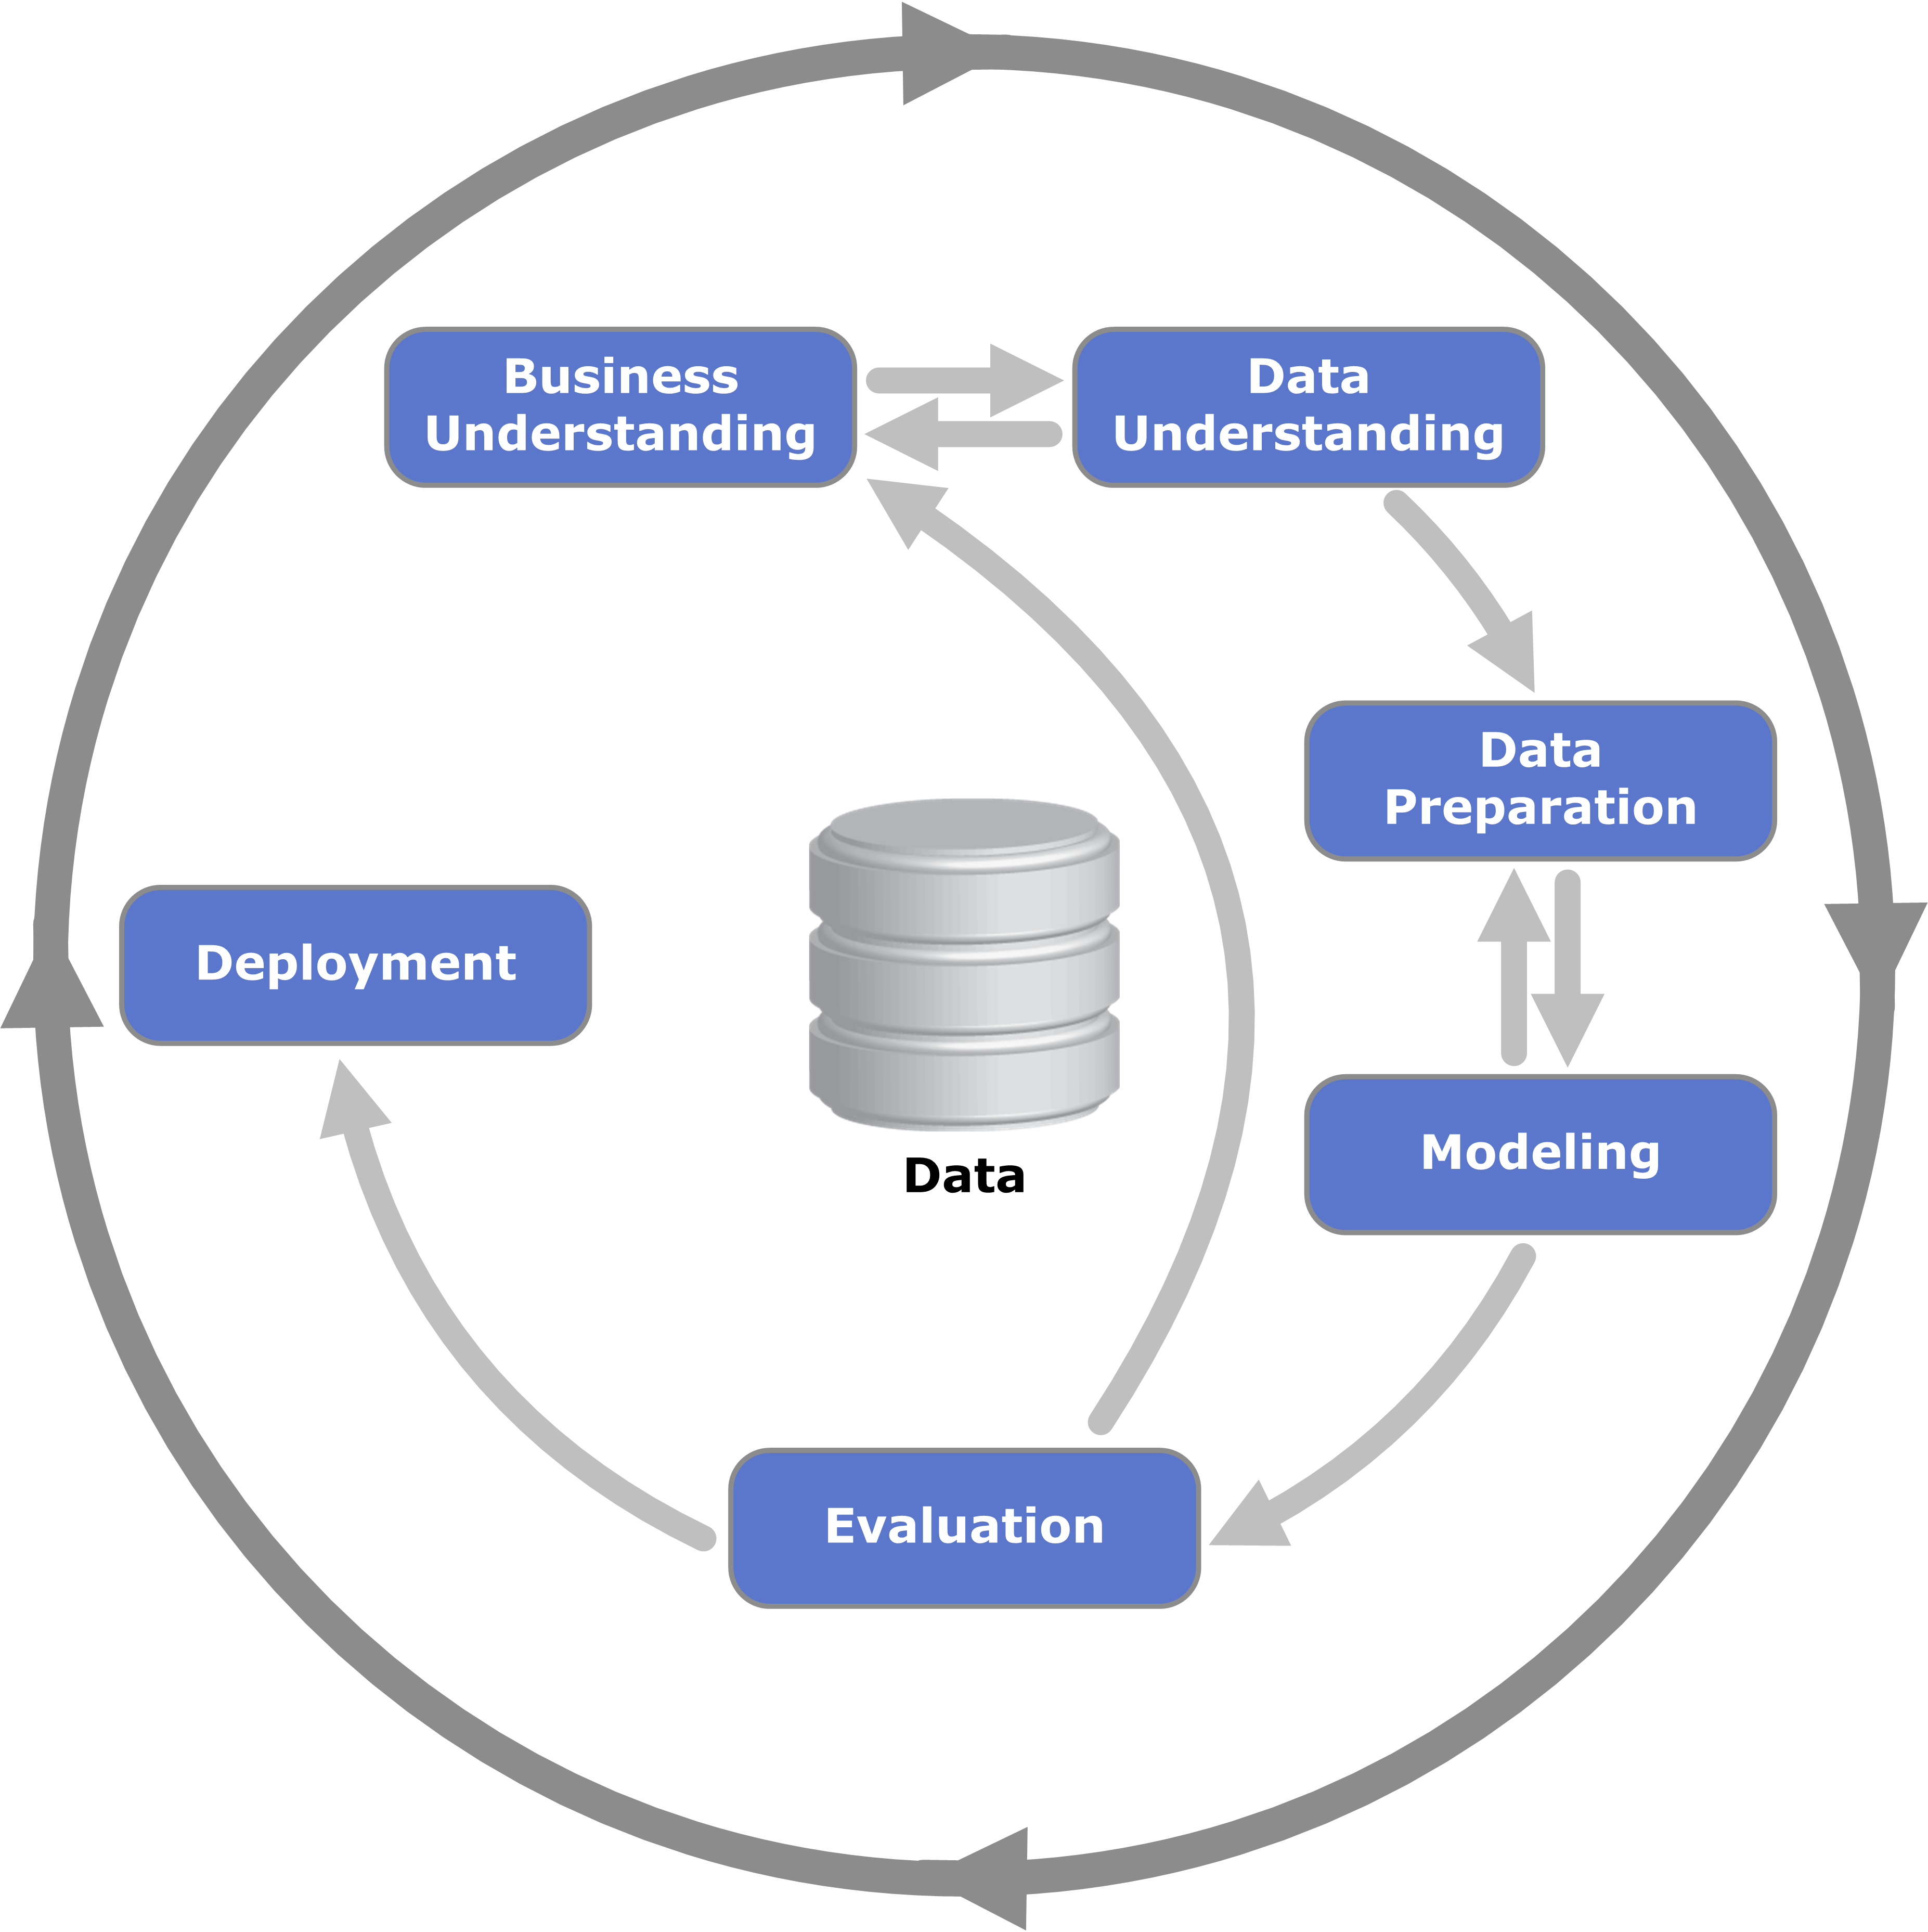
\includegraphics[width=0.45\textwidth]{images/crispdm.png}
\caption{Proses CRISP-DM (Jensen 2012)}
\label{fig:crispdm}
\end{figure}

\begin{table}[!htb]
\caption{Penerapan CRISP-DM pada proyek}
\label{tab:crispdm}
\small
\begin{tabularx}{\textwidth}{@{}p{3.6cm}Xp{1.9cm}@{}}
\toprule
\textbf{Tahap} & \textbf{Penerapan pada proyek} & \textbf{Bab} \\
\midrule
\textit{Business Understanding} & Menentukan tujuan, ukuran popularitas, dan pertanyaan penelitian & I \\
\midrule
\textit{Data Understanding} & Mengeksplorasi struktur dan \textit{key} DBLP, statistik data, dan popularitas konferensi & II, IV, V \\
\midrule
\textit{Data Preparation} & \textit{Preprocessing} lima tahap dan pembentukan dua \textit{transactional database} & IV, VI \\
\midrule
\textit{Modeling} & Apriori, FP-Growth, dan \textit{association rules} & VII, VIII \\
\midrule
\textit{Evaluation} & Validasi hasil, perbandingan performa, dan analisis temporal & IX, X \\
\midrule
\textit{Deployment} & Laporan dan presentasi & XI, XII \\
\bottomrule
\end{tabularx}
\end{table}

\begin{figure}[!htb]
\centering
\figtikz[7cm]{fig-alur-kerja}
\caption{Alur data dan \textit{notebook}}
\label{fig:alur-kerja}
\end{figure}

\section{\textit{Business Understanding}}
Tujuan proyek adalah mengetahui konferensi yang paling aktif dan konferensi yang sering dipilih oleh peneliti yang sama. Popularitas konferensi diukur dari aktivitas publikasi, yaitu jumlah publikasi dan jumlah penulis unik, sedangkan keterkaitan antarkonferensi diukur dari kemunculan bersama pada riwayat publikasi penulis.

\section{\textit{Data Understanding}}
\label{sec:ekstraksi}
Tahap ini terdiri atas tiga kegiatan.
\begin{enumerate}
\item Ekstraksi: \textit{dump} dibaca secara \textit{streaming} dan hanya \textit{record} \texttt{inproceedings} 2015--2025 yang disimpan (2.004.202 \textit{record}).
\item Seleksi: \textit{record} harus bertag \texttt{inproceedings}, ber\textit{key} \texttt{conf/}, dan terbit pada 2015--2025. Syarat \texttt{conf/} ditambahkan karena 3.161 \textit{record} bertag \texttt{inproceedings} berasal dari prosiding acara kecil pada seri jurnal (\texttt{journals/corr}, \texttt{journals/entcs}, dan \texttt{books/sp}) yang menyatu menjadi \textit{venue} palsu dan tidak mungkin mencapai \textit{min\_sup}.
\item Analisis popularitas: pertumbuhan dinyatakan dengan \textit{compound annual growth rate} (CAGR) 2015--2024, dan tahun 2025 tidak dipakai karena datanya belum lengkap. Keselarasan dua peringkat diukur dengan korelasi Spearman, dan dampak penggabungan \textit{workshop} ke konferensi induk diuji dengan menghitung ulang peringkat tanpa \textit{workshop}.
\end{enumerate}

\section{\textit{Data Preparation}}
\label{sec:preprocessing}
\subsection{\textit{Preprocessing}}
Tabel~\ref{tab:prepro} merangkum lima tahap \textit{preprocessing}, yang masing-masing dikerjakan pada salinan data mentah.

\begin{table}[!htb]
\caption{Tahapan \textit{preprocessing}}
\label{tab:prepro}
\small
\begin{tabularx}{\textwidth}{@{}p{3.3cm}XX@{}}
\toprule
\textbf{Tahap} & \textbf{Perlakuan} & \textbf{Alasan} \\
\midrule
Konsistensi tahun & Konversi teks ke bilangan bulat dan validasi rentang 2015--2025 & \texttt{year} bertipe teks pada XML \\
\midrule
\textit{Missing values} & Membuang makalah tanpa penulis & Tidak dapat masuk transaksi dan umumnya bukan makalah \\
\midrule
Seleksi dan normalisasi \textit{venue} & Hanya \textit{key} \texttt{conf/}; \textit{venue} = segmen kedua \textit{key} & Sesuai Subbab~\ref{sec:key}; \textit{booktitle} tidak konsisten \\
\midrule
Duplikat & Membuang \textit{key} ganda, lalu judul, tahun, dan \textit{venue} ganda & Satu makalah tidak boleh terhitung dua kali \\
\midrule
Normalisasi penulis & Normalisasi Unicode NFKC dan spasi; sufiks DBLP dipertahankan; dipecah per penulis & Menyeragamkan nama tanpa menggabungkan orang berbeda \\
\bottomrule
\end{tabularx}
\end{table}

Hasil \textit{preprocessing} disimpan dalam format Parquet, yang lebih kecil dan lebih cepat dibaca daripada CSV serta mempertahankan tipe data. Tiga tabel dihasilkan: \texttt{raw} (2.004.202 makalah), \texttt{clean} (1.997.244 makalah) untuk perhitungan per makalah, dan \texttt{paper\_author} (7.870.902 pasangan makalah-penulis) untuk perhitungan per penulis dan pembentukan transaksi.

\subsection{\textit{Transactional Database}}
Dua \textit{database} dibentuk dari \texttt{paper\_author} dengan \textit{venue} sebagai item (Tabel~\ref{tab:def-db}). Setiap transaksi berupa himpunan \textit{venue} unik, sehingga dua makalah pada \textit{venue} yang sama dalam satu transaksi hanya menghasilkan satu item. Bentuk ini sesuai dengan tujuan analisis, yaitu daftar konferensi tempat penulis menerbitkan makalah, dan jumlah makalah per transaksi tetap tersimpan pada kolom \texttt{n\_paper}.

\begin{table}[!htb]
\caption{Definisi dua \textit{transactional database}}
\label{tab:def-db}
\small
\begin{tabularx}{\textwidth}{@{}p{2.8cm}XX@{}}
\toprule
 & \textbf{\textit{Author-based}} & \textbf{\textit{Author-year-based}} \\
\midrule
Satu transaksi & Satu penulis & Satu kombinasi penulis dan tahun \\
\midrule
Item & \textit{Venue} yang diterbitkan penulis selama 2015--2025 & \textit{Venue} yang diterbitkan penulis pada tahun itu \\
\midrule
Dipakai pada & \textit{Frequent pattern mining} dan \textit{association rules} & Analisis temporal \\
\bottomrule
\end{tabularx}
\end{table}

\subsection{Struktur Data}
\label{sec:struktur-data}
Kedua \textit{database} dibentuk dari satu tabel panjang \texttt{(tid, item)} yang disimpan di disk agar isinya konsisten, lalu diturunkan menjadi dua bentuk di memori (Gambar~\ref{fig:satu-sumber}). Kesetaraan kedua bentuk diperiksa pada jumlah transaksi, jumlah pasangan, ukuran tiap transaksi, dan isi 2.000 transaksi acak. Tabel~\ref{tab:bentuk} membandingkan bentuk yang dipertimbangkan.

\begin{figure}[!htb]
\centering
\figtikz[6.6cm]{fig-satu-sumber}
\caption{Struktur data \textit{transactional database}}
\label{fig:satu-sumber}
\end{figure}

\begin{table}[!htb]
\caption{Bentuk representasi \textit{database} \textit{author-based}}
\label{tab:bentuk}
\small
\begin{tabularx}{\textwidth}{@{}p{2.8cm}XlX@{}}
\toprule
\textbf{Bentuk} & \textbf{Struktur} & \textbf{Memori} & \textbf{Kegunaan} \\
\midrule
Horizontal & \textit{List} \textit{frozenset} berkode integer & 270 MB & Masukan Apriori dan FP-Growth \\
\midrule
\textit{Sparse} CSR & Matriks 0 dan 1 transaksi $\times$ item & 35 MB & Statistik dan validasi \texttt{mlxtend} \\
\midrule
\textit{Dense} & Matriks 0 dan 1 penuh & 8,0 GB & Tidak dibuat \\
\bottomrule
\end{tabularx}
\end{table}

\subsection{Aturan \textit{Mining}}
\label{sec:aturan-mining}
Empat aturan ditetapkan agar hasil konsisten.
\begin{enumerate}
\item Item yang tidak \textit{frequent} dipangkas sebelum \textit{mining}.
\item Penyebut \textit{support} adalah seluruh transaksi, sedangkan transaksi berisi kurang dari dua item \textit{frequent} cukup dilewati untuk \textit{itemset} berukuran dua ke atas.
\item Waktu eksekusi tidak mencakup pemuatan Parquet dan pembentukan \textit{database} horizontal, tetapi mencakup pembentukan FP-\textit{tree} pada FP-Growth.
\item Hasil setiap algoritma divalidasi dengan \texttt{mlxtend} \cite{raschka2018}: \textit{itemset} dan \textit{support} harus identik.
\end{enumerate}

\section{\textit{Modeling}}
Apriori dan FP-Growth dijalankan pada \textit{author-based database}, lalu \textit{association rules} dibangkitkan dari \textit{frequent itemsets} yang dihasilkan. Konfigurasi eksperimen dirangkum pada Tabel~\ref{tab:konfigurasi}.

\begin{table}[!htb]
\caption{Konfigurasi eksperimen}
\label{tab:konfigurasi}
\small
\begin{tabularx}{\textwidth}{@{}p{4.6cm}X@{}}
\toprule
\textbf{Parameter} & \textbf{Nilai} \\
\midrule
\textit{Database} \textit{mining} dan perbandingan performa & \textit{Author-based} (1.821.757 transaksi) \\
\midrule
\textit{min\_sup} & 0,1\%, 0,5\%, 1\%, dan 2\% \\
\midrule
\textit{min\_conf} & 50\% \\
\midrule
Ukuran \textit{rule} & \textit{Support}, \textit{confidence}, dan \textit{lift} \\
\midrule
Pengulangan waktu & Tiga kali per kombinasi, dilaporkan median dan rentangnya \\
\midrule
\textit{Database} analisis temporal & \textit{Author-year-based}, empat periode: 2015--2017, 2018--2020, 2021--2023, dan 2024--2025 \\
\midrule
\textit{min\_sup} analisis temporal & 0,01\%, 0,02\% (utama), dan 0,05\% \\
\bottomrule
\end{tabularx}
\end{table}

\section{\textit{Evaluation}}
Evaluasi mencakup tiga hal. Pertama, validasi hasil kedua algoritma terhadap \texttt{mlxtend}. Kedua, perbandingan Apriori dan FP-Growth berdasarkan jumlah \textit{frequent itemsets}, jumlah \textit{rules}, dan waktu eksekusi pada setiap \textit{min\_sup}. Ketiga, perbandingan \textit{rules} antarperiode pada analisis temporal, yaitu yang bertahan, hilang, dan muncul.

\section{\textit{Deployment}}
Hasil disajikan dalam laporan ini dan presentasi. Seluruh kode dan \textit{notebook} dapat dijalankan ulang berurutan dari \textit{dump} DBLP.

\chapter{HASIL PREPROCESSING}
\label{chap:prepro}

Bab ini memuat jenis publikasi pada \textit{dump}, hasil tiap tahap \textit{preprocessing}, dan statistik \textit{dataset} bersih (\textit{Task} 1).

\section{Jenis publikasi}
\label{sec:hasil-jenis}
Tabel~\ref{tab:jenis} menunjukkan jumlah \textit{record} per jenis publikasi pada seluruh \textit{dump} dan pada periode 2015--2025, dan Gambar~\ref{fig:jenis} menggambarkannya pada skala logaritmik.

\begin{table}[ht]
\caption{Jumlah \textit{record} per jenis publikasi DBLP}
\label{tab:jenis}
\small
\begin{tabularx}{\textwidth}{@{}p{3.2cm}>{\raggedright\arraybackslash}X rrr@{}}
\toprule
\textbf{Jenis} & \textbf{Arti} & \textbf{Seluruh DBLP} & \textbf{2015--2025} & \textbf{Porsi} \\
\midrule
\texttt{article} & Artikel jurnal & 4.527.388 & 2.735.633 & 60,4\% \\
\texttt{www} & Halaman profil penulis & 4.247.510 & 1 & 0,0\% \\
\texttt{inproceedings} & Makalah konferensi dan \textit{workshop} & 4.004.309 & 2.004.202 & 50,1\% \\
\texttt{phdthesis} & Disertasi & 158.395 & 71.290 & 45,0\% \\
\texttt{incollection} & Bab dalam buku & 71.264 & 21.625 & 30,3\% \\
\texttt{proceedings} & Buku prosiding induk & 65.903 & 31.809 & 48,3\% \\
\texttt{data} & \textit{Dataset} & 31.529 & 22.230 & 70,5\% \\
\texttt{book} & Buku & 21.654 & 5.813 & 26,8\% \\
\texttt{mastersthesis} & Tesis magister & 27 & 4 & 14,8\% \\
\midrule
\textbf{Total} & & \textbf{13.127.979} & & \\
\bottomrule
\end{tabularx}
\end{table}

\begin{figure}[ht]
\centering
\figtikz{fig-jenis-publikasi}
\caption{Jumlah \textit{record} per jenis publikasi, seluruh \textit{dump} dibandingkan dengan periode 2015--2025 (skala logaritmik)}
\label{fig:jenis}
\end{figure}

Jenis \texttt{article} dan \texttt{www} menyumbang sekitar 67\% isi \textit{dump}, sedangkan \texttt{inproceedings} hanya 30,5\%. Separuh \texttt{inproceedings} (50,1\%) terbit pada 2015--2025. Jenis \texttt{www} hanya memiliki satu \textit{record} pada periode ini karena itu adalah halaman profil penulis yang umumnya tidak bertahun. Jenis \texttt{proceedings} adalah buku prosiding induk yang dirujuk lewat \texttt{crossref}, bukan makalah.

\section{Hasil preprocessing}
\label{sec:hasil-prepro}
Data berkurang dari 2.004.202 menjadi 1.997.244 makalah, yaitu 6.958 makalah (0,35\%) dibuang dan 99,65\% dipertahankan. Tabel~\ref{tab:dampak} merinci dampak tiap tahap dan Gambar~\ref{fig:alur-seleksi} memperlihatkan alurnya dari seluruh \textit{dump}.

\begin{table}[ht]
\caption{Dampak tiap tahap \textit{preprocessing}}
\label{tab:dampak}
\small
\begin{tabularx}{\textwidth}{@{}>{\raggedright\arraybackslash}X rrr@{}}
\toprule
\textbf{Tahap} & \textbf{Dibuang} & \textbf{Tersisa} & \textbf{Porsi dibuang} \\
\midrule
0. Data mentah (\texttt{inproceedings} 2015--2025) & & 2.004.202 & \\
1. Konsistensi tahun & 0 & 2.004.202 & 0\% \\
2. Makalah tanpa penulis & 2.255 & 2.001.947 & 32\% \\
3. \textit{Key} bukan \texttt{conf/} & 3.161 & 1.998.786 & 45\% \\
4. Duplikat judul, tahun, dan \textit{venue} & 1.542 & 1.997.244 & 22\% \\
5. Normalisasi penulis & 0 & 1.997.244 & 0\% \\
\midrule
\textbf{Total} & \textbf{6.958} & \textbf{1.997.244} & \textbf{100\%} \\
\bottomrule
\end{tabularx}
\end{table}

\begin{figure}[ht]
\centering
\figtikz{fig-alur-seleksi}
\caption{Alur seleksi data dari seluruh \textit{dump} sampai \textit{dataset} bersih}
\label{fig:alur-seleksi}
\end{figure}

Hasil setiap tahap diuraikan berikut ini.

\textbf{Konsistensi tahun.} Seluruh nilai \texttt{year} berupa empat digit dan berada pada 2015--2025 sehingga tidak ada baris yang dibuang. Penyaringan rentang sebenarnya sudah dilakukan saat ekstraksi sehingga tahap ini berfungsi sebagai validasi dan konversi tipe.

\textbf{Missing values.} Makalah tanpa penulis dibuang (2.255 makalah) karena tidak dapat masuk transaksi, dan isinya hampir seluruhnya halaman depan prosiding. Kolom \textit{booktitle} (190 kosong) dan \textit{crossref} (2.471 kosong) dibiarkan karena tidak dipakai, sedangkan \textit{title} dan \textit{year} tidak ada yang kosong.

\textbf{Normalisasi venue.} Seleksi \texttt{conf/} membuang 3.161 makalah, dan penurunan \textit{venue} dari \textit{key} mengubah 8.784 nama \textit{booktitle} menjadi 4.373 \textit{venue}. Sebanyak 1.270 \textit{venue} (29,0\%) memiliki lebih dari satu variasi \textit{booktitle}, dan 377.262 makalah (18,9\%) memakai \textit{booktitle} yang bukan nama dominan \textit{venue}-nya.

\textbf{Duplikat.} Terdapat 1.373 grup makalah dengan judul, tahun, dan \textit{venue} yang sama sehingga 1.542 baris dibuang (0,08\%). Seluruh anggota grup memiliki \textit{key} berbeda, biasanya dengan akhiran huruf (\texttt{...23} dan \texttt{...23a}). Tabel~\ref{tab:duplikat} menunjukkan bahwa sekitar 80\% grup memiliki daftar penulis yang identik sehingga hampir pasti duplikat. Sisanya berupa campuran: makalah sama dengan urutan penulis berbeda, ejaan nama berbeda (\textit{Joaquin} dan \textit{Joaquín}), himpunan bagian penulis, dan judul generik seperti \textit{Preface} (27 grup).

\begin{table}[ht]
\caption{Rincian grup duplikat}
\label{tab:duplikat}
\small
\begin{tabular}{@{}lrr@{}}
\toprule
\textbf{Jenis grup} & \textbf{Grup} & \textbf{Baris dibuang} \\
\midrule
Daftar penulis identik & 1.100 (80,1\%) & 1.121 \\
Daftar penulis berbeda & 273 (19,9\%) & 421 \\
\bottomrule
\end{tabular}
\end{table}

\textbf{Normalisasi penulis.} Normalisasi NFKC dan perapian spasi \textbf{tidak mengubah satu pun} dari 7.870.999 kemunculan nama, dan jumlah nama unik tetap 1.821.757 sebelum dan sesudahnya. DBLP sudah menyajikan nama dalam bentuk yang bersih sehingga tahap ini berfungsi sebagai pengaman. Beberapa temuan lain dicatat.
\begin{enumerate}
\item Sebanyak 97 pasangan makalah-penulis ganda dalam satu makalah dibuang (7.870.999 menjadi 7.870.902).
\item Sebanyak 90.593 nama membawa sufiks disambiguasi DBLP (\textit{Wei Wang 0001}) dan dipertahankan karena menghapusnya menggabungkan orang berbeda.
\item Sebanyak 7.573 kelompok nama (0,42\% dari nama unik) hanya berbeda huruf besar-kecil atau diakritik (\textit{A. Gómez} dan \textit{A. Gomez}). Kelompok ini tidak digabung karena sebagian besar berupa inisial yang sudah ambigu.
\item Masalah sebaliknya lebih berpengaruh: nama umum tanpa sufiks mewakili banyak orang. \textit{Yang Liu} tercatat pada 332 \textit{venue} dan 725 makalah, dan \textit{Wei Wang} pada 280 \textit{venue}.
\end{enumerate}

\section{Statistik dataset bersih}
\label{sec:hasil-statistik}
Tabel~\ref{tab:statistik} merangkum statistik \textit{dataset} setelah \textit{preprocessing}. Seluruh angka dihitung dari tabel Parquet hasil \textit{preprocessing}. Pasangan makalah-penulis hampir empat kali jumlah makalah karena satu makalah memiliki beberapa penulis.

\begin{table}[ht]
\caption{Statistik \textit{dataset} setelah \textit{preprocessing}}
\label{tab:statistik}
\begin{tabular}{@{}lr@{}}
\toprule
\textbf{Statistik} & \textbf{Nilai} \\
\midrule
Total publikasi & 1.997.244 \\
Total penulis unik & 1.821.757 \\
Total konferensi atau \textit{venue} unik & 4.373 \\
Pasangan makalah-penulis & 7.870.902 \\
Penulis per makalah (median dan rata-rata) & 4 dan 3,94 \\
Makalah per penulis (median dan rata-rata) & 1 dan 4,32 \\
Penulis dengan satu makalah & 51,4\% \\
\bottomrule
\end{tabular}
\end{table}

\subsection{Distribusi per tahun}
\label{sec:hasil-tahun}
Gambar~\ref{fig:per-tahun} menunjukkan jumlah publikasi per tahun. Jumlah publikasi naik dari 160.800 pada 2015 ke puncak 213.328 pada 2024, yaitu kenaikan 32,7\% atau CAGR 3,2\% per tahun. Garis tren linear menambah rata-rata 4.796 makalah per tahun. Pada 2020, jumlah turun 8,8\% dan tetap di bawah garis tren sampai 2022, lalu kembali di atasnya pada 2023 (naik 13,1\%). Kaitan penurunan ini dengan pandemi hanya dugaan karena data tidak memuat penyebabnya.

\begin{figure}[ht]
\centering
\figtikz{fig-publikasi-tahun}
\caption{Jumlah publikasi per tahun, 2015--2025}
\label{fig:per-tahun}
\end{figure}

\label{sec:hasil-2025}
Penurunan 6,5\% pada 2025 bukan penurunan aktivitas. Sebanyak 789 konferensi aktif pada 2024 tetapi kosong pada 2025, dan konferensi tersebut menyumbang 49.328 makalah (23,1\% dari total 2024). Ada dua penyebab yang berbeda, terlihat dari pola tahunannya.
\begin{enumerate}
\item Konferensi dua tahunan genap, seperti ECCV (1.638 makalah pada 2020, 0 pada 2021, 2.011 pada 2022, 0 pada 2023, 2.957 pada 2024, dan 0 pada 2025) dan ICPR, memang tidak diadakan pada 2025.
\item Konferensi tahunan yang prosidingnya belum terindeks, seperti IGARSS (2.589 makalah pada 2024), ICCCNT (2.119), dan EMBC (1.386), memiliki data setiap tahun sampai 2024 lalu kosong pada 2025.
\end{enumerate}
Sebaliknya, 322 konferensi kosong pada 2024 tetapi aktif pada 2025 (17.785 makalah), umumnya konferensi dua tahunan ganjil. Jika 789 konferensi yang kosong dikeluarkan, jumlah makalah 2025 berada 21,7\% di atas 2024. Angka ini bukan ukuran pertumbuhan yang adil karena 322 konferensi yang hanya aktif pada 2025 tetap terhitung. Meskipun demikian, angka tersebut cukup untuk menunjukkan bahwa penurunan 6,5\% adalah efek komposisi. Karena itu 2025 digambar dengan arsiran dan tidak dipakai menghitung CAGR maupun garis tren.

\subsection{Distribusi per konferensi}
\label{sec:hasil-konferensi}
Sepuluh konferensi teratas menghasilkan 9,4\% publikasi dan dua puluh teratas 15,6\%. Sebanyak 231 dari 4.373 \textit{venue} (5,3\%) menghasilkan separuh publikasi, dan 1.011 \textit{venue} (23,1\%) menghasilkan 80\%. Median \textit{venue} hanya memiliki 134 makalah selama sebelas tahun, dengan rata-rata 457 dan maksimum 25.455 (NeurIPS). Sebanyak 1.358 \textit{venue} (31,1\%) memiliki kurang dari 50 makalah. Distribusi ini sangat condong ke kanan: sedikit konferensi sangat besar dan banyak konferensi kecil (Gambar~\ref{fig:ukuran-venue}). Sepuluh konferensi terbesar dibahas pada Subbab~\ref{sec:hasil-t2}.

\begin{figure}[ht]
\centering
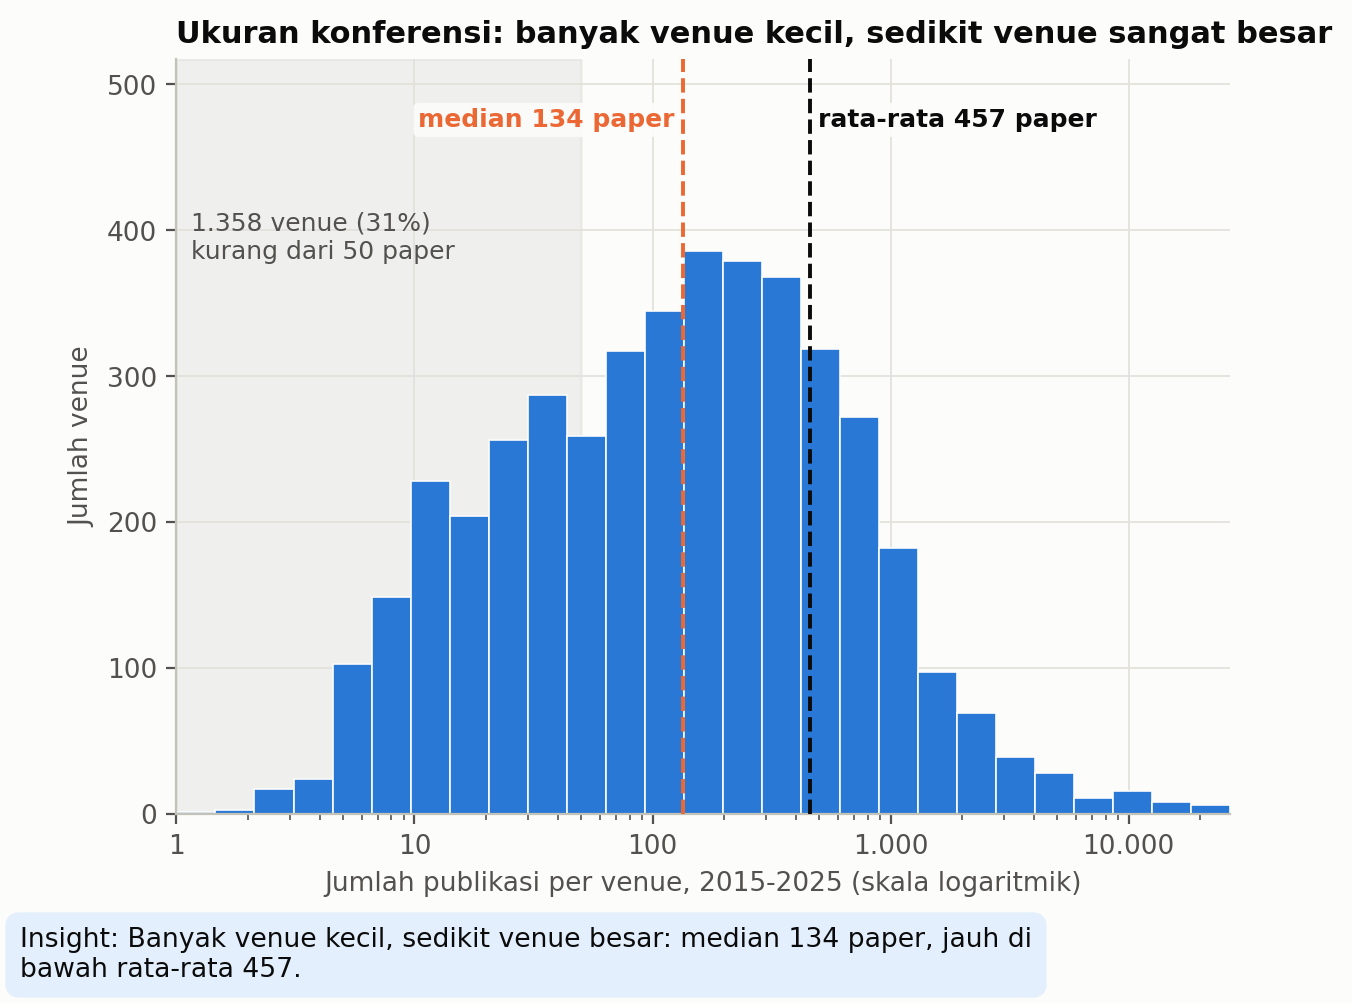
\includegraphics[width=\textwidth]{images/hasil/t1_distribusi_ukuran_venue.png}
\caption{Distribusi ukuran \textit{venue} berdasarkan jumlah makalah}
\label{fig:ukuran-venue}
\end{figure}

\subsection{Distribusi penulis}
\label{sec:hasil-penulis}
Gambar~\ref{fig:waffle} membandingkan porsi penulis dan porsi pasangan makalah-penulis menurut jumlah makalah yang ditulis. Sebanyak 51,4\% penulis hanya menulis satu makalah, tetapi hanya menyumbang 11,9\% pasangan. Sebaliknya, 8,3\% penulis (11 makalah ke atas, 150.894 orang) menyumbang 52,6\% pasangan. Implikasinya, pola konferensi yang muncul bersama kemungkinan lebih banyak dibentuk oleh kelompok kecil penulis yang menerbitkan di banyak konferensi.

\begin{figure}[ht]
\centering
\figtikz{fig-waffle-author}
\caption{Porsi penulis dan porsi pasangan makalah-penulis menurut jumlah makalah per penulis}
\label{fig:waffle}
\end{figure}

\begin{table}[ht]
\caption{Distribusi penulis menurut jumlah makalah}
\label{tab:penulis}
\small
\begin{tabular}{@{}lrrrr@{}}
\toprule
\textbf{Kelompok} & \textbf{Penulis} & \textbf{\% penulis} & \textbf{Pasangan} & \textbf{\% pasangan} \\
\midrule
1 makalah & 936.884 & 51,4\% & 936.884 & 11,9\% \\
2--3 makalah & 434.849 & 23,9\% & 1.015.531 & 12,9\% \\
4--10 makalah & 299.130 & 16,4\% & 1.778.866 & 22,6\% \\
11--50 makalah & 135.073 & 7,4\% & 2.769.731 & 35,2\% \\
lebih dari 50 makalah & 15.821 & 0,9\% & 1.369.890 & 17,4\% \\
\bottomrule
\end{tabular}
\end{table}

\chapter{HASIL \textit{CONFERENCE POPULARITY ANALYSIS}}
\label{chap:popularitas}\label{sec:hasil-t2}

\section{Sepuluh Konferensi Teratas}
\label{sec:hasil-top}
Popularitas diukur dengan dua ukuran. Jumlah publikasi menghitung makalah yang diterbitkan konferensi, sedangkan jumlah penulis unik menghitung orang berbeda yang pernah menerbitkan di sana, dengan satu orang dihitung sekali berapa pun jumlah makalahnya. Kedua ukuran dihitung dari seluruh periode 2015--2025.

Gambar~\ref{fig:top-pub} dan Gambar~\ref{fig:top-author} menunjukkan sepuluh konferensi dengan publikasi terbanyak dan penulis unik terbanyak.
\begin{enumerate}
\item NeurIPS berada di peringkat pertama pada kedua ukuran (25.455 makalah atau 1,27\% \textit{dataset}, dan 57.800 penulis unik), disusul CVPR (22.751; 47.664) dan ICASSP (21.606; 42.057).
\item Delapan dari sepuluh konferensi sama pada kedua daftar. CHI dan ICC hanya masuk pada daftar publikasi, sedangkan ICML (31.896 penulis) dan IROS (31.249) hanya masuk pada daftar penulis unik.
\item Sepuluh konferensi teratas menghasilkan 9,4\% seluruh publikasi dan berasal dari bidang yang beragam, yaitu kecerdasan buatan dan pemrosesan bahasa alami, sinyal dan penginderaan jauh, interaksi manusia-komputer, serta biomedis dan komunikasi.
\end{enumerate}

\begin{figure}[!htb]
\centering
\figtikz[9.2cm]{fig-top10-publikasi}
\caption{Sepuluh konferensi dengan publikasi terbanyak}
\label{fig:top-pub}
\end{figure}

\begin{figure}[!htb]
\centering
\figtikz[9.2cm]{fig-top10-author}
\caption{Sepuluh konferensi dengan penulis unik terbanyak}
\label{fig:top-author}
\end{figure}

\section{Tren Publikasi}
\label{sec:hasil-tren}
Tren dihitung untuk 2015--2024 karena 2025 belum lengkap. Pertumbuhan diringkas dengan \textit{compound annual growth rate} (CAGR), yaitu laju pertumbuhan tahunan rata-rata dari 2015 ke 2024, dan diperlihatkan sebagai kelipatan jumlah makalah.

Gambar~\ref{fig:tren-top10} menunjukkan tren sepuluh konferensi teratas dan Gambar~\ref{fig:cagr} laju pertumbuhannya.
\begin{enumerate}
\item NeurIPS, EMNLP, CVPR, dan AAAI tumbuh 10,2, 7,6, 4,8, dan 3,6 kali dari 2015 ke 2024, jauh di atas CAGR seluruh \textit{dataset} (3,2\%).
\item HCI hampir datar, sedangkan ICC dan EMBC menurun.
\item Porsi sepuluh konferensi teratas terhadap seluruh publikasi naik dari 7,0\% (2015) menjadi 11,7\% (2024), sehingga aktivitas makin terkonsentrasi.
\end{enumerate}

\begin{figure}[!htb]
\centering
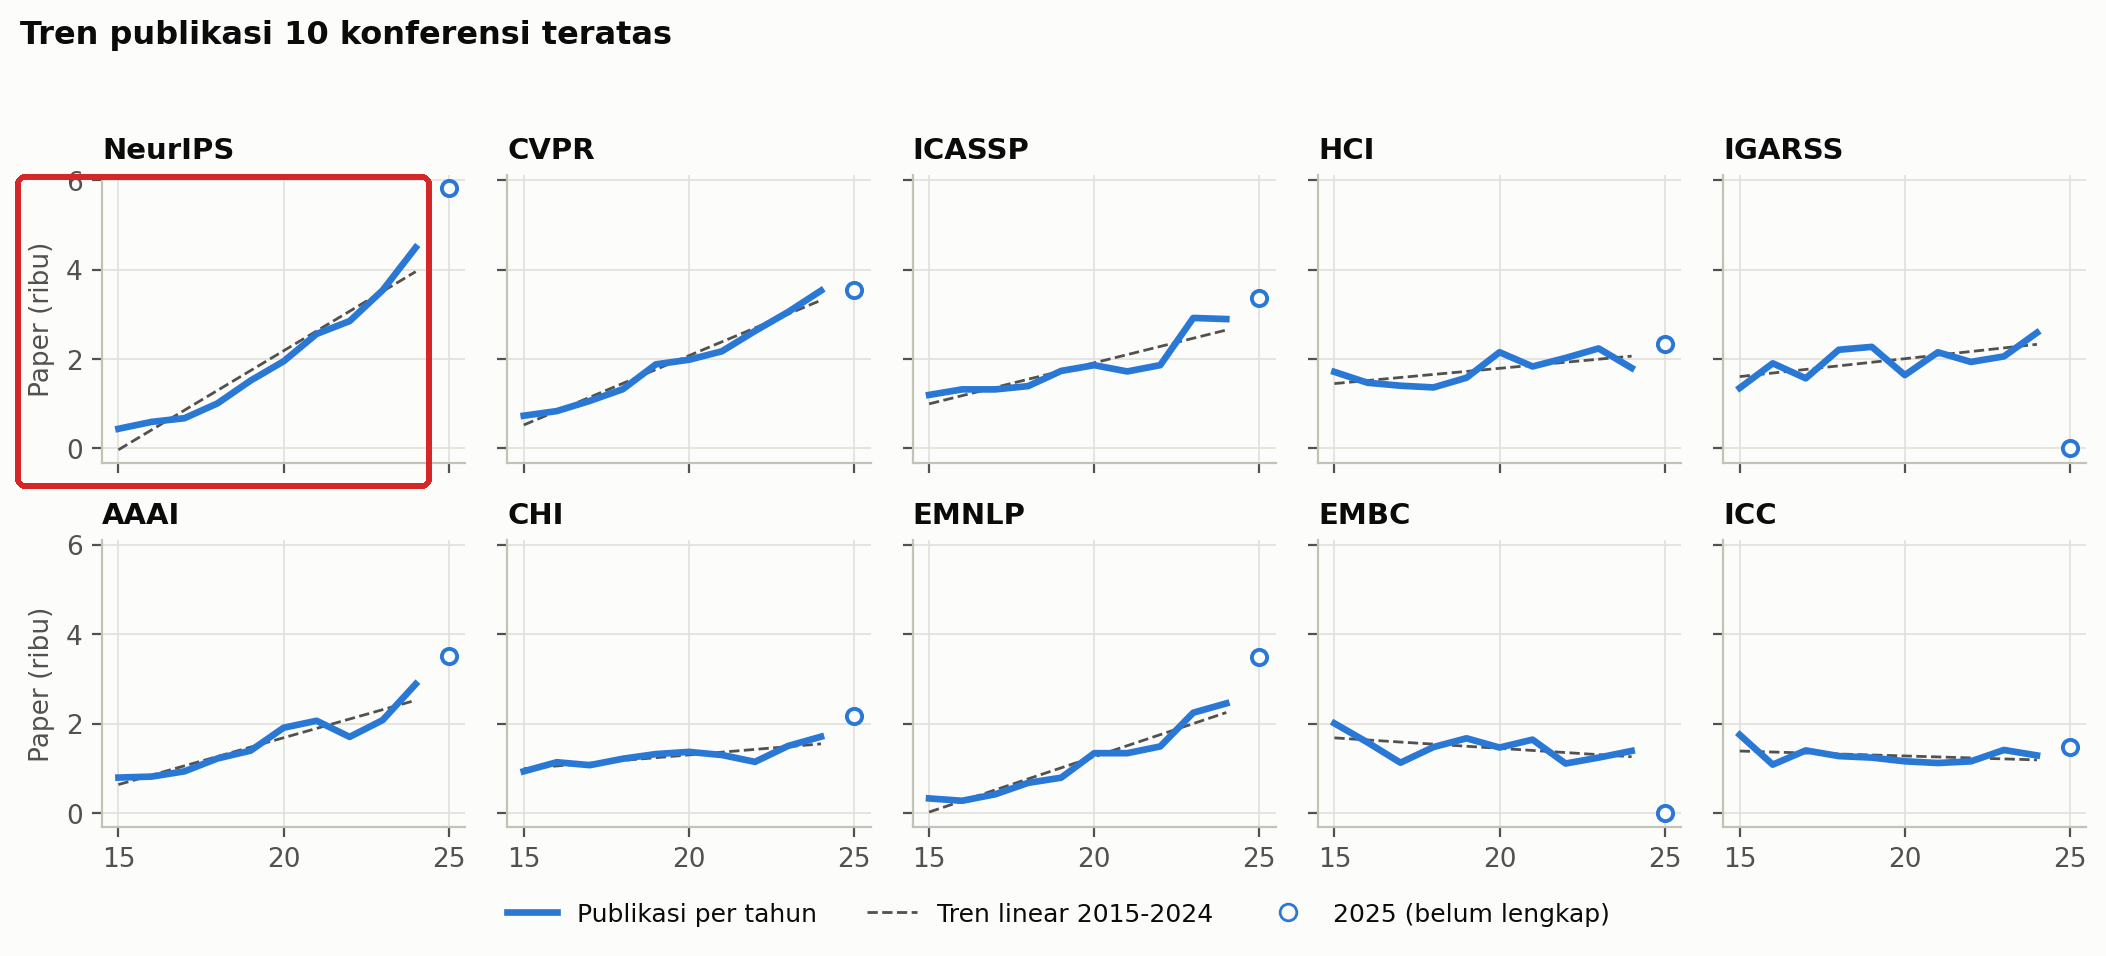
\includegraphics[width=\textwidth]{images/hasil/t2_tren_top10.png}
\caption{Tren publikasi per tahun pada sepuluh konferensi teratas}
\label{fig:tren-top10}
\end{figure}

\begin{figure}[!htb]
\centering
\figtikz[9cm]{fig-cagr-top10}
\caption{Laju pertumbuhan tahunan (CAGR) sepuluh konferensi teratas, 2015--2024}
\label{fig:cagr}
\end{figure}

\section{Perbandingan Peringkat}
\label{sec:hasil-banding}
Tabel~\ref{tab:banding} membandingkan peringkat kedua ukuran, dengan selisih positif berarti naik pada peringkat penulis unik. Kedua peringkat sangat selaras: korelasi Spearman pada 4.373 \textit{venue} mencapai 0,987, dan hampir semua konferensi berada pada sekitar dua penulis unik per makalah (Gambar~\ref{fig:scatter}). Perbedaan terjadi pada peringkat tengah. AAAI dan EMBC naik karena menarik lebih banyak penulis berbeda per makalah, sedangkan CHI dan ICC turun, dengan ICC turun paling jauh (sepuluh ke sembilan belas).

\begin{table}[!htb]
\caption{Perbandingan peringkat publikasi dan penulis unik}
\label{tab:banding}
\small
\begin{tabular*}{\textwidth}{@{\extracolsep{\fill}}@{}lrrr@{}}
\toprule
\textbf{Konferensi} & \textbf{Peringkat publikasi} & \textbf{Peringkat penulis unik} & \textbf{Selisih} \\
\midrule
NeurIPS & 1 & 1 & 0 \\
CVPR & 2 & 2 & 0 \\
ICASSP & 3 & 4 & $-$1 \\
HCI & 4 & 6 & $-$2 \\
IGARSS & 5 & 7 & $-$2 \\
AAAI & 6 & 3 & $+$3 \\
CHI & 7 & 12 & $-$5 \\
EMNLP & 8 & 8 & 0 \\
EMBC & 9 & 5 & $+$4 \\
ICC & 10 & 19 & $-$9 \\
ICML & 12 & 9 & $+$3 \\
IROS & 14 & 10 & $+$4 \\
\bottomrule
\end{tabular*}
\end{table}

\begin{figure}[!htb]
\centering
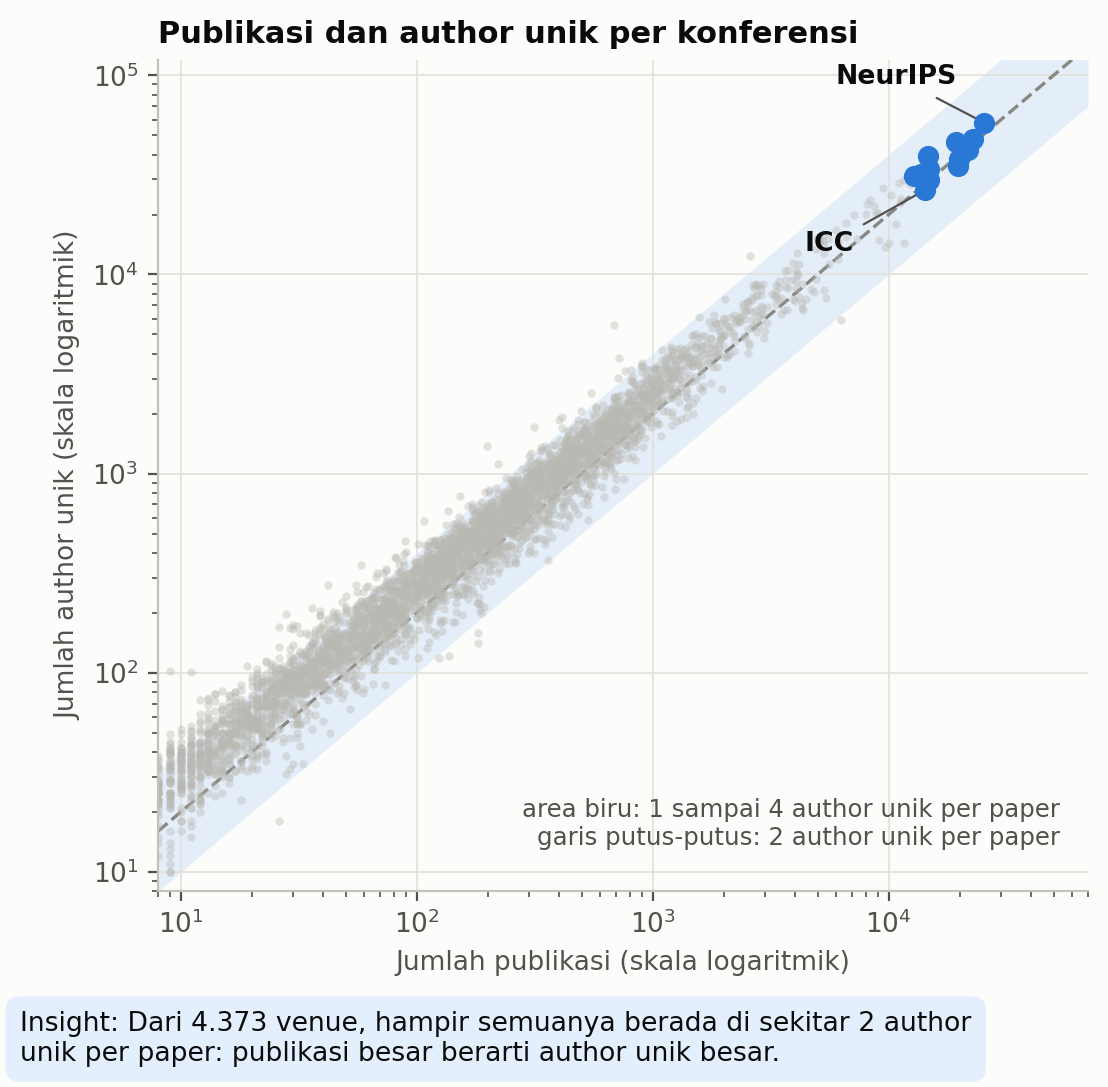
\includegraphics[width=0.62\textwidth]{images/hasil/t2_scatter_publikasi_author.png}
\caption{Publikasi dan penulis unik per konferensi}
\label{fig:scatter}
\end{figure}

\section{Uji Sensitivitas terhadap \textit{Workshop}}
\label{sec:hasil-sensitivitas}
\textit{Workshop} yang memakai \textit{key} konferensi induk ikut terhitung sebagai konferensi induknya (Subbab~\ref{sec:key}). Untuk menguji dampaknya, peringkat dihitung ulang tanpa \textit{workshop} dan acara pendamping, yang dikenali dari kata kunci pada \textit{booktitle} (misalnya \textit{Workshop}, \textit{Extended Abstracts}, \textit{Companion}) dan mencakup 7,2\% makalah. Tabel~\ref{tab:sensitivitas} menunjukkan bahwa peringkat teratas relatif kuat: NeurIPS tetap nomor satu dan delapan dari sepuluh konferensi teratas tetap sama. Konferensi dengan banyak \textit{workshop} paling terpengaruh, yaitu CVPR (\textit{CVPR Workshops}), ICC, dan CHI (\textit{CHI Extended Abstracts}). Karena itu pernyataan bahwa CVPR adalah konferensi terpopuler kedua bergantung pada definisi, dan laporan ini memakai definisi berbasis \textit{key}.

\begin{table}[!htb]
\caption{Peringkat publikasi dengan dan tanpa \textit{workshop}}
\label{tab:sensitivitas}
\small
\begin{tabular*}{\textwidth}{@{\extracolsep{\fill}}@{}lrrr@{}}
\toprule
\textbf{Konferensi} & \textbf{Peringkat awal} & \textbf{Peringkat tanpa \textit{workshop}} & \textbf{Porsi \textit{workshop}} \\
\midrule
NeurIPS & 1 & 1 & 1,1\% \\
CVPR & 2 & 6 & 23,4\% \\
ICASSP & 3 & 2 & 2,2\% \\
CHI & 7 & 29 & 44,0\% \\
ICC & 10 & 18 & 22,8\% \\
ICML & 12 & 9 & 0,6\% \\
\bottomrule
\end{tabular*}
\end{table}

\chapter{HASIL PEMBENTUKAN \textit{TRANSACTIONAL DATABASE}}
\label{chap:transaksi}\label{sec:hasil-t3}

\section{Pembentukan Dua \textit{Database}}
\label{sec:hasil-bentuk}
Dari 7.870.902 pasangan makalah-penulis terbentuk 1.821.757 transaksi pada \textit{author-based} dan 4.085.594 transaksi pada \textit{author-year-based}, dengan 4.373 \textit{venue} sebagai item unik pada keduanya. Gambar~\ref{fig:ilustrasi} mengilustrasikan perbedaannya pada satu penulis dengan 10 makalah di enam \textit{venue} (2021--2024): penulis ini menjadi satu transaksi berisi enam item pada \textit{author-based}, dan empat transaksi berisi tiga, tiga, satu, dan satu item pada \textit{author-year-based}. Dua makalah pada \textit{venue} yang sama dalam satu tahun, yaitu CCE pada 2023 dan ACC pada 2024, hanya menjadi satu item. Cuplikan berkas hasil ada pada Lampiran~\ref{lamp:transaksi}.

\begin{figure}[ht]
\centering
\figtikz{fig-ilustrasi-author}
\caption{Satu penulis pada \textit{author-based} dan \textit{author-year-based}}
\label{fig:ilustrasi}
\end{figure}

\section{Contoh Transaksi}
\label{sec:hasil-contoh}
Tabel~\ref{tab:contoh-a} dan Tabel~\ref{tab:contoh-ay} menunjukkan masing-masing sepuluh transaksi yang dipilih acak (\textit{seed} 42) menurut ukurannya. Transaksi berukuran empat sampai delapan item umumnya berisi \textit{venue} dari bidang yang berdekatan, sedangkan transaksi 25 item (\textit{Haibo Zhang}) mencampur banyak bidang dan kemungkinan menggabungkan beberapa orang bernama sama.

\begin{table}[ht]
\caption{Sepuluh contoh transaksi \textit{author-based}}
\label{tab:contoh-a}
\footnotesize
\begin{tabularx}{\textwidth}{@{}rlrX@{}}
\toprule
\textbf{tid} & \textbf{Author} & \textbf{Item} & \textbf{Isi transaksi} \\
\midrule
338077 & Cheoljoong Park & 1 & ISSCC \\
1245823 & Renann F. Brandao & 2 & LATINCOM, \textit{Image Perception, Observe}\ldots \\
851248 & Satoru Isaka & 3 & CASE, ICDL, SMC \\
466299 & Josef Guggemos & 4 & CSEDU, DeLFI, LTEC, RiE \\
389961 & Solvita Berzisa & 5 & BIR, ICEIS, ICIST, PROFES, SAC \\
808044 & Arun Kumar Thittai & 6 & HEALTHINF, EMBC, ISBI, \textit{Biomedical Applications i}\ldots, SMC, TENCON \\
64961 & Wei Li 0022 & 8 & ACAI, ECCV, ICDE, ICIP, ICPADS, NSDI, PCM, SIGIR \\
391158 & Thierry J. Chaussalet & 10 & BioInfoMed, CBMS, CIBCB, ECMS, HPCC/SmartCity/DSS, ICCS, ICIMTH, INISTA, \textit{IEEE Conf. on}\ldots \\
78397 & Tomás Masarík & 15 & ESA, GD, ICALP, IJCAI, ISAAC, IWOCA, IPEC [iwpec], MFCS, PODC, EC, \ldots{} ($+$5 lagi) \\
25570 & Haibo Zhang & 25 & WISA, ADHIP, AIAM, CACRE, CRC, CSPS, DSA, EEET, EIDWT, EMO, \ldots{} ($+$15 lagi) \\
\bottomrule
\end{tabularx}
\end{table}

\begin{table}[ht]
\caption{Sepuluh contoh transaksi \textit{author-year-based}}
\label{tab:contoh-ay}
\footnotesize
\begin{tabularx}{\textwidth}{@{}rlrrX@{}}
\toprule
\textbf{tid} & \textbf{Author} & \textbf{Tahun} & \textbf{Item} & \textbf{Isi transaksi} \\
\midrule
538906 & Hao Chen 0031 & 2018 & 1 & IJCNN \\
2566923 & Dirk Väth & 2023 & 2 & ACL, EACL \\
1626199 & Ayse Keles & 2024 & 3 & COMPSAC, EUVIP, EXPLIMED@ECAI \\
758263 & Rik Eshuis & 2015 & 4 & ICSOC, PRO-VE, NetWordS, OTM \\
627726 & Tom Mens & 2018 & 5 & BENEVOL, CDVE, ICSME, ICSR [icsr], MSR \\
1534896 & Christian Haubelt & 2016 & 6 & ARCS, CPS Data, EICS, MCSoC, SAMOS, WiMob \\
102172 & Lijie Wen 0001 & 2022 & 7 & COLING, EMNLP, ICASSP, IPDPS, KDD, NAACL-HLT, SIGIR \\
711013 & Syed Ishtiaque Ahmed & 2020 & 8 & CHI, COMPSAC, CSEE\&T, COMPASS, \textit{Graphics Interface}, ICTD, ICWSM, PDC \\
136050 & Javier Del Ser & 2020 & 10 & CEC, COMPSAC, CW, GECCO Companion, ICCS, IDEAL, IJCNN, ITSC, SOCO, SSCI \\
44703 & Feng Li & 2016 & 14 & CDC, CLSW, GECCO Companion, HCC, ICASSP, ICIC, IGARSS, INFOCOM, ISNN, IJCRS, \ldots{} ($+$4 lagi) \\
\bottomrule
\end{tabularx}
\end{table}

\section{Statistik dan Distribusi}
\label{sec:hasil-statistik-tx}
Tabel~\ref{tab:statistik-tx} merangkum statistik kedua \textit{database}, dan Gambar~\ref{fig:komposisi} menunjukkan distribusi item per transaksi.
\begin{enumerate}
\item \textit{Author-year-based} memiliki 2,24 kali lebih banyak transaksi, karena penulis yang aktif beberapa tahun menjadi beberapa transaksi, tetapi transaksinya lebih kecil (rata-rata 1,59 item dibanding 2,66).
\item Mayoritas transaksi hanya berisi satu item (58,4\% dan 71,0\%). Transaksi seperti ini tidak dapat membentuk pasangan, tetapi tetap masuk penyebut \textit{support}.
\item Distribusinya berekor panjang: rata-rata jauh di atas median (satu item), dan transaksi terbesar (332 dan 85 item) berasal dari \textit{Yang Liu}, nama umum yang menggabungkan banyak orang.
\end{enumerate}

\begin{table}[ht]
\caption{Statistik kedua \textit{transactional database}}
\label{tab:statistik-tx}
\small
\begin{tabular*}{\textwidth}{@{\extracolsep{\fill}}@{}lrr@{}}
\toprule
\textbf{Statistik} & \textbf{\textit{Author-based}} & \textbf{\textit{Author-year-based}} \\
\midrule
Jumlah transaksi & 1.821.757 & 4.085.594 \\
Item unik & 4.373 & 4.373 \\
Item per transaksi: median dan rata-rata & 1 dan 2,66 & 1 dan 1,59 \\
Item per transaksi: persentil 99 dan maksimum & 20 dan 332 & 7 dan 85 \\
Transaksi berisi 1 item & 58,4\% & 71,0\% \\
Transaksi berisi minimal 2 item & 41,6\% & 29,0\% \\
\bottomrule
\end{tabular*}
\end{table}

\begin{figure}[ht]
\centering
\figtikz{fig-komposisi-transaksi}
\caption{Komposisi ukuran transaksi pada kedua \textit{database}}
\label{fig:komposisi}
\end{figure}

\section{Perbedaan Kedua Representasi}
\label{sec:hasil-banding-repr}
Pada \textit{author-based}, dua \textit{venue} dianggap muncul bersama jika seorang penulis pernah menerbitkan di keduanya kapan saja pada 2015--2025. Pada \textit{author-year-based}, keduanya harus diterbitkan pada tahun yang sama. Tabel~\ref{tab:banding-repr} membandingkan pasangan antar-\textit{venue} dengan \textit{support} minimal 0,1\% pada \textit{author-based} (574 \textit{venue}).
\begin{enumerate}
\item \textit{Support} pasangan turun median 0,29 kali pada \textit{author-year-based}. Penyebabnya hampir seluruhnya penyebut: jumlah transaksi yang memuat pasangan hanya turun ke 0,65 kali, sedangkan jumlah transaksi \textit{database} naik 2,24 kali (0,65 dibagi 2,24 sama dengan sekitar 0,29). \textit{Min\_sup} yang sama karena itu berarti ambang absolut yang lebih tinggi.
\item Sekitar 23\% pasangan tidak pernah muncul pada \textit{author-year-based}, yaitu pasangan lintas tahun.
\item Urutan teratas relatif terjaga (Tabel~\ref{tab:top-pasangan}): 18 dari 20 pasangan teratas sama dan korelasi peringkatnya 0,892. ACL + EMNLP justru naik dari peringkat 6 ke 3 karena penulis yang konsisten menerbitkan di keduanya setiap tahun dihitung berulang.
\item Konferensi dua tahunan berselang tidak dapat berpasangan. ICCV dan ECCV memiliki 10.051 transaksi bersama pada \textit{author-based}, tetapi nol pada \textit{author-year-based} (Tabel~\ref{tab:iccv}).
\end{enumerate}

\begin{table}[ht]
\caption{Perbandingan pasangan \textit{venue} pada kedua representasi}
\label{tab:banding-repr}
\small
\begin{tabular*}{\textwidth}{@{\extracolsep{\fill}}@{}lr@{}}
\toprule
\textbf{Ukuran} & \textbf{Nilai} \\
\midrule
Pasangan yang muncul sedikitnya sekali, \textit{author-based} dan \textit{author-year-based} & 157.402 dan 120.937 \\
Median rasio \textit{support} (\textit{author-year} per \textit{author}) pada 100 pasangan teratas & 0,29 \\
Irisan 20 pasangan teratas dan korelasi peringkat Spearman & 18 dari 20 dan 0,892 \\
\bottomrule
\end{tabular*}
\end{table}

\begin{table}[ht]
\caption{Lima pasangan \textit{venue} teratas pada \textit{author-based} dan padanannya pada \textit{author-year-based}}
\label{tab:top-pasangan}
\footnotesize
\begin{tabularx}{\textwidth}{@{}>{\raggedright\arraybackslash}X rrrrrr@{}}
\toprule
\textbf{Pasangan} & \textbf{Trans. (A)} & \textbf{\textit{Support} (A)} & \textbf{Trans. (AY)} & \textbf{\textit{Support} (AY)} & \textbf{Rank AY} & \textbf{Rasio trans.} \\
\midrule
ICML + NeurIPS & 18.503 & 1,02\% & 17.719 & 0,43\% & 1 & 0,96 \\
ICLR + NeurIPS & 17.852 & 0,98\% & 16.438 & 0,40\% & 2 & 0,92 \\
AAAI + NeurIPS & 15.973 & 0,88\% & 12.281 & 0,30\% & 6 & 0,77 \\
CVPR + NeurIPS & 15.640 & 0,86\% & 14.485 & 0,35\% & 4 & 0,93 \\
CVPR + ICCV & 15.441 & 0,85\% & 12.359 & 0,30\% & 5 & 0,80 \\
\bottomrule
\end{tabularx}
\end{table}

\begin{table}[ht]
\caption{Transaksi \textit{author-year-based} yang memuat ICCV dan ECCV per tahun}
\label{tab:iccv}
\footnotesize
\setlength{\tabcolsep}{3.5pt}
\begin{tabular*}{\textwidth}{@{\extracolsep{\fill}}@{}lrrrrrrrrrrr@{}}
\toprule
 & \textbf{2015} & \textbf{2016} & \textbf{2017} & \textbf{2018} & \textbf{2019} & \textbf{2020} & \textbf{2021} & \textbf{2022} & \textbf{2023} & \textbf{2024} & \textbf{2025} \\
\midrule
ICCV & 1.543 & 0 & 1.959 & 0 & 3.627 & 0 & 5.971 & 0 & 8.439 & 0 & 15.260 \\
ECCV & 0 & 1.986 & 0 & 3.770 & 0 & 6.001 & 0 & 7.869 & 0 & 11.930 & 0 \\
\bottomrule
\end{tabular*}
\end{table}

Kedua representasi menjawab pertanyaan yang berbeda, dengan kelebihan dan keterbatasan masing-masing untuk \textit{frequent pattern mining}.
\begin{enumerate}
\item \textit{Author-based} berisi transaksi yang lebih kaya (41,6\% berisi minimal dua item) dan menangkap asosiasi lintas waktu, tetapi tidak memiliki dimensi waktu dan bebannya terkonsentrasi pada transaksi besar (0,1\% transaksi menanggung 27,8\% pasangan yang dapat dibentuk).
\item \textit{Author-year-based} mengikat kemunculan bersama pada waktu yang sama dan dapat dipotong per periode, tetapi 71,0\% transaksinya hanya satu item sehingga \textit{support} pasangan rendah dan pasangan lintas tahun hilang.
\item \textit{Author-based} dipilih untuk \textit{Task} 4 dan \textit{Task} 5 karena riwayat publikasi mencakup seluruh periode, dan \textit{author-year-based} dipilih untuk Bagian E karena memiliki dimensi tahun.
\end{enumerate}
Model himpunan tidak menyimpan jumlah makalah per \textit{venue}: 38,3\% makalah pada \textit{author-based} dan 17,4\% pada \textit{author-year-based} tidak menambah item baru.

\chapter{HASIL \textit{FREQUENT PATTERN MINING}}
\label{chap:fpm}\label{sec:hasil-t4}
Bab ini memuat hasil \textit{Task} 4 pada \textit{author-based database}, dimulai dengan Apriori \cite{agrawal1994} (Subbab~\ref{sec:hasil-t4-apriori} sampai \ref{sec:jawab-t4-apriori}), lalu FP-Growth \cite{han2000} (Subbab~\ref{sec:hasil-t4-fp-validasi} sampai \ref{sec:jawab-t4-fp}). Perbandingan performa kedua algoritma dibahas pada Bab~\ref{sec:hasil-t6}.

% Sisi Apriori dari Task 4 (Harfhan). Diinput pada bab4-task4-7.tex sebelum sisi FP-Growth.
\section{Implementasi dan validasi Apriori}
\label{sec:hasil-t4-apriori}
Apriori \cite{agrawal1994} diimplementasikan sendiri (\texttt{src/apriori.py}) dan dijalankan pada \textit{author-based database} dengan empat \textit{min\_sup} yang sama dengan FP-Growth. Setiap tingkat $k$ membentuk kandidat $C_k$ dari \textit{frequent} $(k-1)$-\textit{itemset} $L_{k-1}$. Langkah \textit{join} menggabungkan dua \textit{itemset} yang memiliki $k-2$ item pertama yang sama, lalu langkah \textit{prune} membuang kandidat yang memiliki subset berukuran $k-1$ tidak \textit{frequent}. \textit{Support} kandidat yang tersisa dihitung dengan satu pemindaian, dan proses berhenti ketika $L_k$ kosong.

Pra-pemrosesan dibuat sama dengan FP-Growth agar perbandingan waktu pada Bab~\ref{sec:hasil-t6} adil. Item yang tidak \textit{frequent} dipangkas setelah pemindaian pertama, transaksi dengan kurang dari dua item \textit{frequent} dilewati tetapi tetap dihitung pada penyebut \textit{support}, dan transaksi yang identik setelah pemangkasan digabung lalu dihitung sekali dengan bobotnya. Pada \textit{min\_sup} 0,1\%, langkah ini memadatkan 1.821.757 transaksi menjadi 315.694 transaksi unik berbobot, berasal dari 536.543 transaksi yang memuat minimal dua item \textit{frequent}. Ambang \textit{min count} dihitung dengan fungsi yang sama dengan FP-Growth.

Penghitungan kandidat memakai satu optimasi. Untuk setiap transaksi, item yang tidak ada pada kandidat mana pun dibuang lebih dulu, lalu dipilih cara yang lebih murah: mengenumerasi seluruh subset berukuran $k$ dari transaksi dan mencocokkannya dengan himpunan kandidat, atau memeriksa setiap kandidat sebagai subset transaksi. Optimasi ini diperlukan karena transaksi terpanjang memuat 187 item \textit{frequent} pada 0,1\%, sehingga enumerasi subset berukuran tiga saja menghasilkan lebih dari satu juta kombinasi untuk satu transaksi.

Implementasi diuji dengan \texttt{pytest} pada tiga lapis. Contoh sembilan transaksi pada buku \textcite{han2012} menghasilkan $|C_1| = 5$, $|C_2| = 10$, dan $|C_3| = 2$ setelah \textit{prune}, beserta 13 \textit{frequent itemsets}, sama dengan buku. Enam \textit{dataset} acak menghasilkan \textit{itemset} dan \textit{count} yang sama dengan \textit{brute force}, dan transaksi kosong terbukti tetap dihitung pada penyebut. Pada data asli, hasil keempat \textit{min\_sup} identik dengan \texttt{mlxtend} dan dengan FP-Growth (Tabel~\ref{tab:t4-apriori-validasi}).

\begin{table}[ht]
\caption{Validasi Apriori terhadap \texttt{mlxtend} dan FP-Growth pada \textit{author-based}}
\label{tab:t4-apriori-validasi}
\small
\begin{tabular}{@{}lrrrrrc@{}}
\toprule
\textbf{\textit{min\_sup}} & \textbf{Apriori} & \textbf{\texttt{mlxtend}} & \textbf{FP-Growth} & \textbf{Hilang} & \textbf{Berlebih} & \textbf{Identik} \\
\midrule
0,1\% & 1.514 & 1.514 & 1.514 & 0 & 0 & ya \\
0,5\% & 88 & 88 & 88 & 0 & 0 & ya \\
1\% & 30 & 30 & 30 & 0 & 0 & ya \\
2\% & 6 & 6 & 6 & 0 & 0 & ya \\
\bottomrule
\end{tabular}
\end{table}

Karena \textit{itemset} dan \textit{count}-nya identik, Tabel~\ref{tab:t4-ukuran}, \ref{tab:t4-top10}, \ref{tab:t4-pasangan}, dan \ref{tab:t4-triple} pada subbab FP-Growth berlaku juga untuk Apriori dan tidak diulang di sini. Bab ini membahas hal yang khas Apriori, yaitu jumlah kandidat yang harus dihitung.

\section{Kandidat dan \textit{frequent itemsets} per tingkat}
\label{sec:hasil-t4-apriori-kandidat}
Tabel~\ref{tab:t4-apriori-level} merinci setiap tingkat Apriori pada keempat \textit{min\_sup}: jumlah kandidat $|C_k|$, jumlah \textit{frequent itemsets} $|L_k|$, dan persentase kandidat yang ternyata \textit{frequent}. Kandidat tingkat 1 adalah seluruh 4.373 \textit{venue}. Waktu per tingkat berasal dari satu kali eksekusi pada \textit{notebook} \texttt{03\_apriori} dan hanya dipakai untuk melihat porsi biaya setiap tingkat. Pengukuran waktu berulang ada pada Bab~\ref{sec:hasil-t6}.

\begin{table}[ht]
\caption{Kandidat dan \textit{frequent itemsets} per tingkat Apriori}
\label{tab:t4-apriori-level}
\small
\begin{tabular}{@{}lrrrrr@{}}
\toprule
\textbf{\textit{min\_sup}} & \textbf{$k$} & \textbf{Kandidat $|C_k|$} & \textbf{\textit{Frequent} $|L_k|$} & \textbf{\textit{Frequent}/kandidat} & \textbf{Waktu (detik)} \\
\midrule
0,1\% & 1 & 4.373 & 574 & 13,13\% & 1,60 \\
 & 2 & 164.451 & 393 & 0,24\% & 2,98 \\
 & 3 & 1.228 & 348 & 28,34\% & 0,78 \\
 & 4 & 337 & 159 & 47,18\% & 0,40 \\
 & 5 & 54 & 37 & 68,52\% & 0,16 \\
 & 6 & 5 & 3 & 60,00\% & 0,10 \\
\midrule
0,5\% & 1 & 4.373 & 66 & 1,51\% & 1,31 \\
 & 2 & 2.145 & 21 & 0,98\% & 0,37 \\
 & 3 & 13 & 1 & 7,69\% & 0,05 \\
\midrule
1\% & 1 & 4.373 & 29 & 0,66\% & 0,87 \\
 & 2 & 406 & 1 & 0,25\% & 0,12 \\
\midrule
2\% & 1 & 4.373 & 6 & 0,14\% & 0,81 \\
 & 2 & 15 & 0 & 0,00\% & 0,00 \\
\bottomrule
\end{tabular}
\end{table}

\begin{figure}[ht]
\centering
\figtikz{fig-t4-apriori-kandidat}
\caption{Kandidat dan \textit{frequent itemsets} per tingkat Apriori pada \textit{min\_sup} 0,1\%}
\label{fig:t4-apriori-kandidat}
\end{figure}

Gambar~\ref{fig:t4-apriori-kandidat} memperlihatkan bahwa biaya Apriori terkumpul di tingkat 2. Pada 0,1\% terdapat 574 item \textit{frequent}, sehingga $C_2$ berisi seluruh $574 \times 573 / 2 = 164.451$ pasangan. Langkah \textit{prune} tidak dapat membuang satu pun pasangan karena setiap subset berukuran satu sudah \textit{frequent}. Hanya 393 pasangan (0,24\%) yang ternyata \textit{frequent}, dan tingkat 2 memakan sekitar separuh total waktu Apriori. Mulai tingkat 3, langkah \textit{prune} bekerja efektif. Dari 393 pasangan hanya terbentuk 1.228 kandidat, dan persentase kandidat yang \textit{frequent} naik dari 28\% pada tingkat 3 menjadi 69\% pada tingkat 5. Secara keseluruhan, Apriori menghitung 166.075 kandidat berukuran dua ke atas untuk menemukan 940 \textit{itemset}, atau 177 kali jumlah \textit{itemset} yang akhirnya \textit{frequent}.

Pada \textit{min\_sup} yang lebih tinggi, $L_1$ jauh lebih kecil (66, 29, dan 6 item) sehingga $C_2$ ikut mengecil secara kuadratik (2.145, 406, dan 15). Waktu kemudian didominasi tingkat 1, yaitu pemindaian pertama 1,8 juta transaksi beserta pemangkasan dan penggabungannya, yang biayanya hampir tetap untuk semua \textit{min\_sup}. Dari 2\% ke 0,1\%, jumlah item \textit{frequent} naik 96 kali, tetapi kandidat tingkat 2 naik sekitar 11.000 kali. Pola ini sesuai dengan sebaran berekor panjang pada Subbab~\ref{sec:hasil-statistik-tx}: banyak konferensi cukup besar untuk lolos sebagai item tunggal, tetapi sangat sedikit pasangan yang lolos.

\section{Jawaban pertanyaan \textit{Task} 4 (sisi Apriori)}
\label{sec:jawab-t4-apriori}
\textbf{\textit{Frequent itemsets}.} Apriori menemukan 1.514, 88, 30, dan 6 \textit{frequent itemsets} pada \textit{min\_sup} 0,1\%, 0,5\%, 1\%, dan 2\%, identik dengan \texttt{mlxtend} dan FP-Growth.

\textbf{1-, 2-, dan 3-\textit{itemset}, sepuluh teratas, dan kombinasi teratas.} Sama dengan FP-Growth (Subbab~\ref{sec:jawab-t4-fp}) karena kedua algoritma menghasilkan \textit{itemset} dan \textit{count} yang sama.

\textbf{Pengaruh \textit{min\_sup}.} Selain mengurangi jumlah \textit{itemset}, menaikkan \textit{min\_sup} mengurangi kandidat Apriori secara tajam, dari 166.075 kandidat berukuran dua ke atas pada 0,1\% menjadi 2.158, 406, dan 15 pada 0,5\%, 1\%, dan 2\%. Pada 0,1\%, hampir seluruh kandidat berada di tingkat 2 dan hanya 0,24\% yang \textit{frequent}.

\textbf{Interpretasi.} Pola konferensinya sama dengan Subbab~\ref{sec:hasil-t4-fp-interpretasi}. Dari sisi algoritma, ekor panjang data DBLP adalah kasus yang berat bagi tingkat 2 Apriori tetapi ringan bagi tingkat berikutnya, karena pasangan \textit{frequent} sedikit dan terkumpul pada beberapa bidang.

% Sisi FP-Growth dari Task 4 (Mahesa). Sisi Apriori ada pada bab4-task4-apriori.tex.

\section{Implementasi dan validasi FP-Growth}
\label{sec:hasil-t4-fp-validasi}
FP-Growth diimplementasikan sendiri (\texttt{src/fpgrowth.py}) dan mengikuti empat aturan pada Subbab~\ref{sec:aturan-mining}. Item yang tidak \textit{frequent} dipangkas setelah pemindaian pertama. Transaksi dengan kurang dari dua item \textit{frequent} tidak dimasukkan ke FP-\textit{tree} karena tidak dapat memuat kombinasi, tetapi tetap dihitung pada penyebut \textit{support}, dan \textit{support} 1-\textit{itemset} diambil dari pemindaian pertama. Transaksi yang identik setelah pemangkasan digabung dan dimasukkan sekali dengan bobotnya. Urutan item di pohon adalah \textit{count} menurun, lalu kode item menaik, sehingga hasilnya deterministik. Ambang dihitung sebagai bilangan bulat terkecil $c$ dengan $c/N \ge$ \textit{min\_sup}, yaitu 1.822, 9.109, 18.218, dan 36.436 penulis untuk \textit{min\_sup} 0,1\%, 0,5\%, 1\%, dan 2\%.

Implementasi diuji dengan \texttt{pytest} pada tiga lapis. Contoh sembilan transaksi pada buku \textcite{han2012} menghasilkan bentuk FP-\textit{tree} dan 13 \textit{frequent itemsets} yang sama dengan buku. Enam belas \textit{dataset} acak menghasilkan \textit{itemset} dan \textit{count} yang sama dengan perhitungan \textit{brute force} atas seluruh subset. Pada data asli, hasil keempat \textit{min\_sup} identik dengan \texttt{mlxtend} \cite{raschka2018} (Tabel~\ref{tab:t4-validasi}).

\begin{table}[ht]
\caption{Validasi FP-Growth terhadap \texttt{mlxtend} pada \textit{author-based}}
\label{tab:t4-validasi}
\small
\begin{tabular}{@{}lrrrrrc@{}}
\toprule
\textbf{\textit{min\_sup}} & \textbf{FP-Growth} & \textbf{\texttt{mlxtend}} & \textbf{Hilang} & \textbf{Berlebih} & \textbf{\textit{Count} beda} & \textbf{Identik} \\
\midrule
0,1\% & 1.514 & 1.514 & 0 & 0 & 0 & ya \\
0,5\% & 88 & 88 & 0 & 0 & 0 & ya \\
1\% & 30 & 30 & 0 & 0 & 0 & ya \\
2\% & 6 & 6 & 0 & 0 & 0 & ya \\
\bottomrule
\end{tabular}
\end{table}

\section{\textit{Frequent itemsets} pada empat \textit{min\_sup}}
\label{sec:hasil-t4-fp-jumlah}
Tabel~\ref{tab:t4-ukuran} dan Gambar~\ref{fig:t4-ukuran} menunjukkan jumlah \textit{frequent itemsets} menurut ukurannya. Pada \textit{min\_sup} 0,1\% ditemukan 1.514 \textit{itemset}, terdiri atas 574 1-\textit{itemset}, 393 pasangan, 348 \textit{triple}, dan 199 \textit{itemset} berisi empat sampai enam konferensi. Pada 0,5\% tersisa 88 \textit{itemset} dengan satu \textit{triple}, pada 1\% tersisa 30 \textit{itemset} dengan satu pasangan, dan pada 2\% hanya enam konferensi tunggal. Perkiraan pada Subbab~\ref{sec:hasil-support-item} terkonfirmasi: \textit{min\_sup} 2\% tidak menghasilkan satu pun pasangan.

\begin{table}[ht]
\caption{Jumlah \textit{frequent itemsets} FP-Growth menurut ukuran}
\label{tab:t4-ukuran}
\small
\begin{tabular}{@{}lrrrrrrr@{}}
\toprule
\textbf{\textit{min\_sup}} & \textbf{\textit{Min count}} & \textbf{Total} & \textbf{1 item} & \textbf{2 item} & \textbf{3 item} & \textbf{4--6 item} & \textbf{Terpanjang} \\
\midrule
0,1\% & 1.822 & 1.514 & 574 & 393 & 348 & 199 & 6 \\
0,5\% & 9.109 & 88 & 66 & 21 & 1 & 0 & 3 \\
1\% & 18.218 & 30 & 29 & 1 & 0 & 0 & 2 \\
2\% & 36.436 & 6 & 6 & 0 & 0 & 0 & 1 \\
\bottomrule
\end{tabular}
\end{table}

\begin{figure}[ht]
\centering
\figtikz{fig-t4-itemset-ukuran}
\caption{Jumlah \textit{frequent itemsets} menurut ukuran dan \textit{min\_sup}}
\label{fig:t4-ukuran}
\end{figure}

\section{Sepuluh \textit{itemset} dengan \textit{support} tertinggi}
\label{sec:hasil-t4-fp-top10}
Pada \textit{min\_sup} 0,1\%, 0,5\%, dan 1\%, sepuluh \textit{itemset} dengan \textit{support} tertinggi sama persis dan seluruhnya berupa konferensi tunggal (Tabel~\ref{tab:t4-top10}). Pada 2\% hanya enam konferensi pertama yang lolos, karena IGARSS (35.229 penulis) berada di bawah ambang 36.436. Tidak ada kombinasi yang masuk sepuluh besar karena pasangan teratas, ICML dan NeurIPS, hanya didukung 18.503 penulis, lebih sedikit dari konferensi ke-10, IROS (31.249 penulis).

\begin{table}[ht]
\caption{Sepuluh \textit{itemset} dengan \textit{support} tertinggi (\textit{min\_sup} 0,1\%, 0,5\%, dan 1\%)}
\label{tab:t4-top10}
\small
\begin{tabular}{@{}rlrr@{}}
\toprule
\textbf{\#} & \textbf{\textit{Itemset}} & \textbf{Penulis} & \textbf{\textit{Support}} \\
\midrule
1 & NeurIPS & 57.800 & 3,17\% \\
2 & CVPR & 47.664 & 2,62\% \\
3 & AAAI & 46.437 & 2,55\% \\
4 & ICASSP & 42.057 & 2,31\% \\
5 & EMBC & 39.318 & 2,16\% \\
6 & HCI & 37.884 & 2,08\% \\
7 & IGARSS & 35.229 & 1,93\% \\
8 & EMNLP & 33.954 & 1,86\% \\
9 & ICML & 31.896 & 1,75\% \\
10 & IROS & 31.249 & 1,72\% \\
\bottomrule
\end{tabular}
\end{table}

\section{Pengaruh \textit{min\_sup}}
\label{sec:hasil-t4-fp-minsup}
Jumlah \textit{itemset} turun 17,2 kali dari 0,1\% ke 0,5\% (1.514 menjadi 88) dan 252 kali dari 0,1\% ke 2\% (1.514 menjadi 6). \textit{Itemset} besar hilang lebih dulu: ukuran empat ke atas hanya ada pada 0,1\%, \textit{triple} hilang setelah 0,5\%, dan pasangan hilang setelah 1\%. Penyebabnya adalah sebaran transaksi yang berekor panjang (Subbab~\ref{sec:hasil-statistik-tx}). Sebanyak 58,4\% penulis hanya menerbitkan di satu \textit{venue} sehingga hanya sebagian kecil transaksi yang dapat memuat kombinasi, dan \textit{support} sebuah kombinasi jauh lebih kecil dari \textit{support} konferensi penyusunnya. Akibatnya, hanya \textit{min\_sup} 0,1\% yang menghasilkan pola kombinasi yang cukup kaya untuk dianalisis. Pada 1\% dan 2\% hasilnya praktis hanya mengulang peringkat popularitas \textit{Task} 2, dan \textit{Task} 5 memakai hasil 0,1\% sebagai dasar utama.

\section{Kombinasi konferensi yang paling sering muncul bersama}
\label{sec:hasil-t4-fp-kombinasi}
Hasil pada 0,1\% memuat seluruh hasil pada \textit{min\_sup} yang lebih tinggi sehingga kombinasi teratas diambil dari sana. Tabel~\ref{tab:t4-pasangan} dan Gambar~\ref{fig:t4-pasangan} menunjukkan sepuluh pasangan teratas, dengan kolom \textit{min\_sup} tertinggi tempat pasangan itu masih \textit{frequent}. Pasangan ini sama dengan pratinjau pada Tabel~\ref{tab:top-pasangan}, kini sebagai hasil \textit{mining}. ICML dan NeurIPS adalah satu-satunya pasangan yang masih \textit{frequent} pada 1\%.

\begin{table}[ht]
\caption{Sepuluh pasangan konferensi teratas (\textit{min\_sup} 0,1\%)}
\label{tab:t4-pasangan}
\small
\begin{tabular}{@{}rlrrr@{}}
\toprule
\textbf{\#} & \textbf{Pasangan} & \textbf{Penulis} & \textbf{\textit{Support}} & \textbf{\textit{Frequent} sampai} \\
\midrule
1 & ICML + NeurIPS & 18.503 & 1,02\% & 1\% \\
2 & ICLR + NeurIPS & 17.852 & 0,98\% & 0,5\% \\
3 & AAAI + NeurIPS & 15.973 & 0,88\% & 0,5\% \\
4 & CVPR + NeurIPS & 15.640 & 0,86\% & 0,5\% \\
5 & CVPR + ICCV & 15.441 & 0,85\% & 0,5\% \\
6 & ACL + EMNLP & 14.557 & 0,80\% & 0,5\% \\
7 & CVPR + ECCV & 13.752 & 0,75\% & 0,5\% \\
8 & ICLR + ICML & 12.947 & 0,71\% & 0,5\% \\
9 & AAAI + CVPR & 12.169 & 0,67\% & 0,5\% \\
10 & ICRA + IROS & 11.860 & 0,65\% & 0,5\% \\
\bottomrule
\end{tabular}
\end{table}

\begin{figure}[ht]
\centering
\figtikz{fig-t4-pasangan}
\caption{Sepuluh pasangan konferensi teratas pada \textit{min\_sup} 0,1\%}
\label{fig:t4-pasangan}
\end{figure}

Tabel~\ref{tab:t4-triple} menunjukkan sepuluh \textit{triple} teratas. ICLR, ICML, dan NeurIPS (10.413 penulis) adalah satu-satunya \textit{triple} yang masih \textit{frequent} pada 0,5\%. NeurIPS muncul pada empat dari sepuluh pasangan teratas dan delapan dari sepuluh \textit{triple} teratas. \textit{Itemset} terpanjang berisi enam konferensi, yaitu AAAI, CVPR, ECCV, ICCV, ICLR, dan NeurIPS (2.005 penulis), disusul CVPR, ECCV, ICCV, ICLR, ICML, dan NeurIPS (1.849) serta AAAI, CVPR, ECCV, ICCV, ACM Multimedia, dan NeurIPS (1.827). Seluruh 40 \textit{itemset} berukuran lima atau enam hanya melibatkan 14 konferensi, dan NeurIPS ada pada 35 di antaranya.

\begin{table}[ht]
\caption{Sepuluh \textit{triple} konferensi teratas (\textit{min\_sup} 0,1\%)}
\label{tab:t4-triple}
\small
\begin{tabular}{@{}rlrr@{}}
\toprule
\textbf{\#} & \textbf{\textit{Triple}} & \textbf{Penulis} & \textbf{\textit{Support}} \\
\midrule
1 & ICLR + ICML + NeurIPS & 10.413 & 0,57\% \\
2 & CVPR + ECCV + ICCV & 8.474 & 0,47\% \\
3 & CVPR + ICCV + NeurIPS & 8.407 & 0,46\% \\
4 & AAAI + ICML + NeurIPS & 7.585 & 0,42\% \\
5 & AAAI + ICLR + NeurIPS & 7.371 & 0,40\% \\
6 & AAAI + CVPR + NeurIPS & 7.301 & 0,40\% \\
7 & CVPR + ECCV + NeurIPS & 7.272 & 0,40\% \\
8 & CVPR + ICLR + NeurIPS & 7.157 & 0,39\% \\
9 & AAAI + CVPR + ICCV & 6.477 & 0,36\% \\
10 & CVPR + ICML + NeurIPS & 6.259 & 0,34\% \\
\bottomrule
\end{tabular}
\end{table}

\section{Popularitas dan keterhubungan}
\label{sec:hasil-t4-fp-keterhubungan}
Konferensi yang besar belum tentu sering dipasangkan dengan konferensi lain. Dari 574 konferensi yang \textit{frequent} pada 0,1\%, hanya 105 yang muncul pada minimal satu pasangan \textit{frequent}. Tabel~\ref{tab:t4-keterhubungan} membandingkan sepuluh konferensi terbesar. AAAI, NeurIPS, ICASSP, dan CVPR masing-masing termasuk dalam 34 sampai 44 pasangan \textit{frequent}, sedangkan EMBC, IGARSS, dan HCI hanya dalam empat, empat, dan satu pasangan. Dua kolom terakhir menjelaskan penyebabnya. Penulis NeurIPS, CVPR, dan ICASSP biasanya menerbitkan di enam konferensi, dan hanya 10,3\% sampai 11,6\% yang menerbitkan di satu konferensi saja. Penulis EMBC, HCI, dan IGARSS biasanya hanya menerbitkan di satu atau dua konferensi, dan 37,4\% sampai 54,2\% tidak pernah menerbitkan di konferensi lain. Penulis yang menerbitkan di tempat lain pun tersebar ke banyak konferensi berbeda sehingga tidak ada pasangan yang mencapai 1.822 penulis.

\begin{table}[ht]
\caption{Keterhubungan sepuluh konferensi terbesar pada \textit{min\_sup} 0,1\%}
\label{tab:t4-keterhubungan}
\small
\begin{tabularx}{\textwidth}{@{}lrr>{\raggedleft\arraybackslash}X>{\raggedleft\arraybackslash}X@{}}
\toprule
\textbf{Konferensi} & \textbf{Penulis} & \textbf{Pasangan \textit{frequent}} & \textbf{Penulis yang hanya di konferensi ini} & \textbf{Median konferensi per penulis} \\
\midrule
NeurIPS & 57.800 & 42 & 11,6\% & 6 \\
CVPR & 47.664 & 34 & 10,3\% & 6 \\
AAAI & 46.437 & 44 & 8,5\% & 8 \\
ICASSP & 42.057 & 41 & 10,6\% & 6 \\
EMBC & 39.318 & 4 & 37,4\% & 2 \\
HCI & 37.884 & 1 & 40,8\% & 2 \\
IGARSS & 35.229 & 4 & 54,2\% & 1 \\
EMNLP & 33.954 & 25 & 11,1\% & 7 \\
ICML & 31.896 & 24 & 8,4\% & 7 \\
IROS & 31.249 & 14 & 16,4\% & 4 \\
\bottomrule
\end{tabularx}
\end{table}

\section{Interpretasi}
\label{sec:hasil-t4-fp-interpretasi}
Nama bidang pada subbab ini, yaitu \textit{machine learning}, \textit{computer vision}, NLP, robotika, dan kecerdasan buatan umum, adalah pengetahuan umum penulis laporan, bukan atribut hasil \textit{mining}. Nama itu dicocokkan dengan judul prosiding pada data DBLP (\texttt{venue\_proceedings.csv}), misalnya \textit{Neural Information Processing Systems}, \textit{Computer Vision and Pattern Recognition}, \textit{Computational Linguistics}, \textit{Robotics and Automation}, dan \textit{Artificial Intelligence}.

\textbf{Kombinasi yang lolos ambang berasal dari bidang yang sama.} Pasangan teratas mengelompok menjadi \textit{machine learning} (ICML, ICLR, NeurIPS), \textit{computer vision} (CVPR, ICCV, ECCV), NLP (ACL, EMNLP), dan robotika (ICRA, IROS). Kombinasi lintas bidang yang lolos hanya terjadi antara \textit{machine learning}, \textit{computer vision}, dan AAAI, misalnya CVPR dan NeurIPS (15.640 penulis).

\textbf{NeurIPS menjadi titik temu.} NeurIPS ada pada sebagian besar pasangan, \textit{triple}, dan \textit{itemset} panjang teratas, dan \textit{itemset} berisi lima atau enam konferensi hanya terbentuk di sekitar \textit{machine learning}, \textit{computer vision}, dan AAAI.

\textbf{Popularitas berbeda dengan keterhubungan.} Konferensi besar seperti EMBC, IGARSS, dan HCI hampir tidak membentuk pasangan \textit{frequent}, sedangkan ICASSP terhubung dengan 41 konferensi lain. Pertanyaan apakah konferensi terpopuler juga memiliki asosiasi terkuat dijawab dengan \textit{lift} pada Bab~\ref{sec:hasil-t5}, karena \textit{support} pasangan yang tinggi dapat muncul hanya karena kedua konferensinya besar.

\textbf{Batas tafsiran.} \textit{Support} hanya mengukur seberapa sering kombinasi muncul. Kombinasi lintas bidang dapat saja banyak secara total tetapi tersebar ke banyak pasangan kecil yang tidak lolos ambang 1.822 penulis, sehingga hasil ini tidak membuktikan bahwa penulis jarang berpindah bidang. Selain itu, 291 transaksi dengan 100 konferensi atau lebih hampir seluruhnya milik nama umum tanpa nomor disambiguasi (Subbab~\ref{sec:hasil-statistik-tx}). Transaksi ini menyumbang median 3,0\% \textit{count} pasangan dan 3,9\% \textit{count} \textit{triple}. Tanpa transaksi tersebut, 109 dari 1.514 \textit{itemset} pada 0,1\% (7\%) jatuh di bawah ambang, tetapi sepuluh pasangan teratas hanya berkurang 0,8\% sampai 1,8\% (ICML dan NeurIPS dari 18.503 menjadi 18.348). Kesimpulan utama tidak berubah, dan hasil dilaporkan apa adanya.

\section{Jawaban pertanyaan \textit{Task} 4 (sisi FP-Growth)}
\label{sec:jawab-t4-fp}
\textbf{\textit{Frequent itemsets}.} FP-Growth menemukan 1.514, 88, 30, dan 6 \textit{frequent itemsets} pada \textit{min\_sup} 0,1\%, 0,5\%, 1\%, dan 2\%, identik dengan \texttt{mlxtend}.

\textbf{1-, 2-, dan 3-\textit{itemset}.} Berturut-turut 574, 393, dan 348 pada 0,1\%; 66, 21, dan 1 pada 0,5\%; 29, 1, dan 0 pada 1\%; serta 6, 0, dan 0 pada 2\%. Pada 0,1\% juga terdapat 199 \textit{itemset} berisi empat sampai enam konferensi.

\textbf{Sepuluh \textit{itemset} teratas.} Seluruhnya konferensi tunggal, dipimpin NeurIPS (57.800 penulis, \textit{support} 3,17\%), CVPR (47.664), dan AAAI (46.437).

\textbf{Pengaruh \textit{min\_sup}.} Jumlah \textit{itemset} turun 17,2 kali dari 0,1\% ke 0,5\% dan 252 kali dari 0,1\% ke 2\%, dan \textit{itemset} besar hilang lebih dulu. Hanya 0,1\% yang menghasilkan pola kombinasi yang cukup kaya.

\textbf{Kombinasi yang paling sering muncul bersama.} ICML dan NeurIPS (18.503 penulis, \textit{support} 1,02\%) untuk pasangan, ICLR, ICML, dan NeurIPS (10.413) untuk \textit{triple}, serta AAAI, CVPR, ECCV, ICCV, ICLR, dan NeurIPS (2.005) sebagai \textit{itemset} terpanjang.

\textbf{Interpretasi.} Kombinasi yang lolos ambang mengelompok per bidang dengan NeurIPS sebagai titik temu, dan popularitas sebuah konferensi tidak menjamin keterhubungannya dengan konferensi lain.


\chapter{HASIL \textit{ASSOCIATION RULE MINING}}
\label{chap:rules}

\chapter{PERBANDINGAN PERFORMA ALGORITMA}
\label{chap:performa}

\chapter{ANALISIS ASOSIASI TEMPORAL}
\label{chap:temporal}\label{sec:hasil-e}
% Bagian E: analisis asosiasi temporal (Mahesa, notebook 07_temporal).
Bab ini membandingkan pola asosiasi konferensi pada empat periode, yaitu 2015--2017, 2018--2020, 2021--2023, dan 2024--2025, menggunakan \textit{author-year-based database} (Bab~\ref{sec:hasil-t3}). Setiap periode diperlakukan sebagai \textit{database} tersendiri: transaksinya adalah pasangan (penulis, tahun) pada periode itu, dan penyebut \textit{support} adalah seluruh transaksi periode tersebut. \textit{Mining} memakai FP-Growth \cite{han2000} yang sudah divalidasi pada Subbab~\ref{sec:hasil-t4-fp-validasi}, dan \textit{rules} dibangkitkan dengan \textit{min\_conf} 50\% seperti \textit{Task} 5.

\section{Data per periode dan pemilihan \textit{min\_sup}}
\label{sec:hasil-e-data}
Tabel~\ref{tab:e-periode} menunjukkan keempat periode memiliki ukuran yang sebanding dan porsi transaksi berisi minimal dua konferensi yang mirip. Periode 2024--2025 hanya dua tahun dan data 2025 belum lengkap, tetapi karena \textit{support} dihitung relatif terhadap jumlah transaksi periode itu sendiri, perbedaan ukuran tidak langsung mengubah \textit{support}.

\begin{table}[ht]
\caption{Transaksi dan jumlah \textit{rules} per periode}
\label{tab:e-periode}
\small
\begin{tabular}{@{}lrrrrrr@{}}
\toprule
 & & & & \multicolumn{3}{c}{\textbf{\textit{Rules} pada \textit{min\_sup}}} \\
\cmidrule(lr){5-7}
\textbf{Periode} & \textbf{Transaksi} & \textbf{$\geq$ 2 konf.} & \textbf{$\geq$ 20 konf.} & \textbf{0,01\%} & \textbf{0,02\%} & \textbf{0,05\%} \\
\midrule
2015--2017 & 922.051 & 29,2\% & 137 & 70 & 17 & 2 \\
2018--2020 & 1.080.824 & 28,2\% & 272 & 130 & 32 & 4 \\
2021--2023 & 1.195.907 & 28,1\% & 511 & 480 & 113 & 25 \\
2024--2025 & 886.812 & 30,8\% & 582 & 7.741 & 1.874 & 282 \\
\bottomrule
\end{tabular}
\end{table}

\textit{Min\_sup} yang dipakai pada \textit{Task} 4 terlalu tinggi untuk \textit{database} ini. Sebanyak 71\% transaksi \textit{author-year} hanya berisi satu konferensi, sehingga pada \textit{min\_sup} 0,1\% tiga periode pertama hanya menghasilkan 1, 0, dan 3 \textit{rules}. Karena itu dipakai tiga ambang yang lebih rendah, yaitu 0,01\%, 0,02\%, dan 0,05\%. Ketiganya dijalankan, lalu satu ambang dipilih sebagai ambang utama dengan kriteria yang ditetapkan sebelum melihat polanya: setiap periode harus memiliki minimal 15 \textit{rules}, dan minimal 80\% \textit{rules} setiap periode harus lolos uji ketahanan.

Uji ketahanan mengulang \textit{mining} setelah transaksi berisi 20 konferensi atau lebih dalam satu tahun dikosongkan, dengan penyebut tetap. Transaksi seperti ini sebagian besar berasal dari nama umum yang menggabungkan beberapa orang (Subbab~\ref{sec:hasil-statistik-tx}). Tabel~\ref{tab:e-tahan} menunjukkan porsi \textit{rules} yang tetap ditemukan.

\begin{table}[ht]
\caption{Porsi \textit{rules} yang tetap ditemukan tanpa transaksi berisi 20 konferensi atau lebih}
\label{tab:e-tahan}
\small
\begin{tabular}{@{}lrrrr@{}}
\toprule
\textbf{\textit{min\_sup}} & \textbf{2015--2017} & \textbf{2018--2020} & \textbf{2021--2023} & \textbf{2024--2025} \\
\midrule
0,01\% & 96\% & 100\% & 93\% & 64\% \\
0,02\% & 94\% & 100\% & 98\% & 67\% \\
0,05\% & 100\% & 100\% & 96\% & 78\% \\
\bottomrule
\end{tabular}
\end{table}

Tidak ada ambang yang memenuhi kedua kriteria karena periode 2024--2025 selalu di bawah 80\%. Ambang 0,05\% juga tidak memenuhi syarat jumlah \textit{rules} (2 dan 4 \textit{rules} pada dua periode awal). Karena tanpa \textit{rules} tidak ada yang dapat dibandingkan, jumlah \textit{rules} tetap dijadikan syarat, dan di antara ambang yang memenuhinya dipilih ketahanan terbaik, yaitu \textbf{0,02\%}. Pada tiga periode pertama ketahanannya 94\% sampai 100\%, sehingga hanya \textit{rules} 2024--2025 yang perlu dibaca hati-hati.

\section{\textit{Frequent itemsets} per periode}
\label{sec:hasil-e-fpm}
Pada 0,02\%, jumlah \textit{itemset} berisi dua konferensi atau lebih adalah 279, 376, 662, dan 2.380 dari periode pertama sampai terakhir, dan \textit{itemset} berisi empat konferensi atau lebih naik dari 1 menjadi 710. Sebaliknya, jumlah konferensi tunggal yang \textit{frequent} turun dari 1.600 menjadi 1.266, padahal ambang \textit{count} 2024--2025 paling rendah (178 transaksi). Penulis makin terkumpul pada konferensi yang sama, dan konferensi itu makin sering muncul bersama dalam satu tahun.

Tabel~\ref{tab:e-pasangan} menunjukkan lima pasangan teratas setiap periode. Pada 2015--2017, pasangan teratas tersebar di telekomunikasi, kendali, robotika, dan komunikasi optik. Hanya satu dari sepuluh pasangan teratas periode ini (AAAI + IJCAI) yang memuat AAAI, NeurIPS, ICML, ICLR, ACL, atau EMNLP. Pada 2024--2025, sembilan dari sepuluh pasangan teratas memuat salah satu konferensi itu, dan pengecualiannya hanya CVPR + ICCV. \textit{Support} ICLR + NeurIPS naik dari 0,18\% pada 2018--2020 menjadi 1,04\%, sedangkan GLOBECOM + ICC turun dari peringkat pertama ke luar sepuluh besar.

\begin{table}[ht]
\caption{Lima pasangan konferensi dengan \textit{support} tertinggi per periode (\textit{min\_sup} 0,02\%)}
\label{tab:e-pasangan}
\footnotesize
\setlength{\tabcolsep}{4pt}
\begin{tabular}{@{}rllll@{}}
\toprule
\textbf{\#} & \textbf{2015--2017} & \textbf{2018--2020} & \textbf{2021--2023} & \textbf{2024--2025} \\
\midrule
1 & GLOBECOM + ICC & CVPR + ECCV & ICML + NeurIPS & ICLR + NeurIPS \\
2 & ACC + CDC & GLOBECOM + ICC & ACL + EMNLP & ICML + NeurIPS \\
3 & ICRA + IROS & ICML + NeurIPS & CVPR + ICCV & CVPR + NeurIPS \\
4 & ECOC + OFC & ICRA + IROS & ICLR + NeurIPS & ACL + EMNLP \\
5 & GLOBECOM + VTC Fall & AAAI + IJCAI & CVPR + NeurIPS & ICLR + ICML \\
\bottomrule
\end{tabular}
\end{table}

\section{\textit{Association rules} per periode}
\label{sec:hasil-e-rules}
Jumlah \textit{rules} naik tajam menuju 2024--2025 pada ketiga ambang (Tabel~\ref{tab:e-periode} dan Gambar~\ref{fig:e-rules}). Median \textit{lift} pada 0,02\% turun dari 49,1 dan 49,2 menjadi 28,0 dan 20,2. \textit{Rules} baru berpusat pada konferensi besar, dan seperti pada Subbab~\ref{sec:hasil-t5-lift}, \textit{rule} yang menuju konferensi besar memiliki \textit{lift} lebih rendah. \textit{Rule} satu-ke-satu hampir tidak ada (2, 1, 1, dan 0): dalam satu tahun, menerbitkan di satu konferensi jarang cukup untuk memprediksi konferensi lain dengan \textit{confidence} 50\%.

\begin{figure}[ht]
\centering
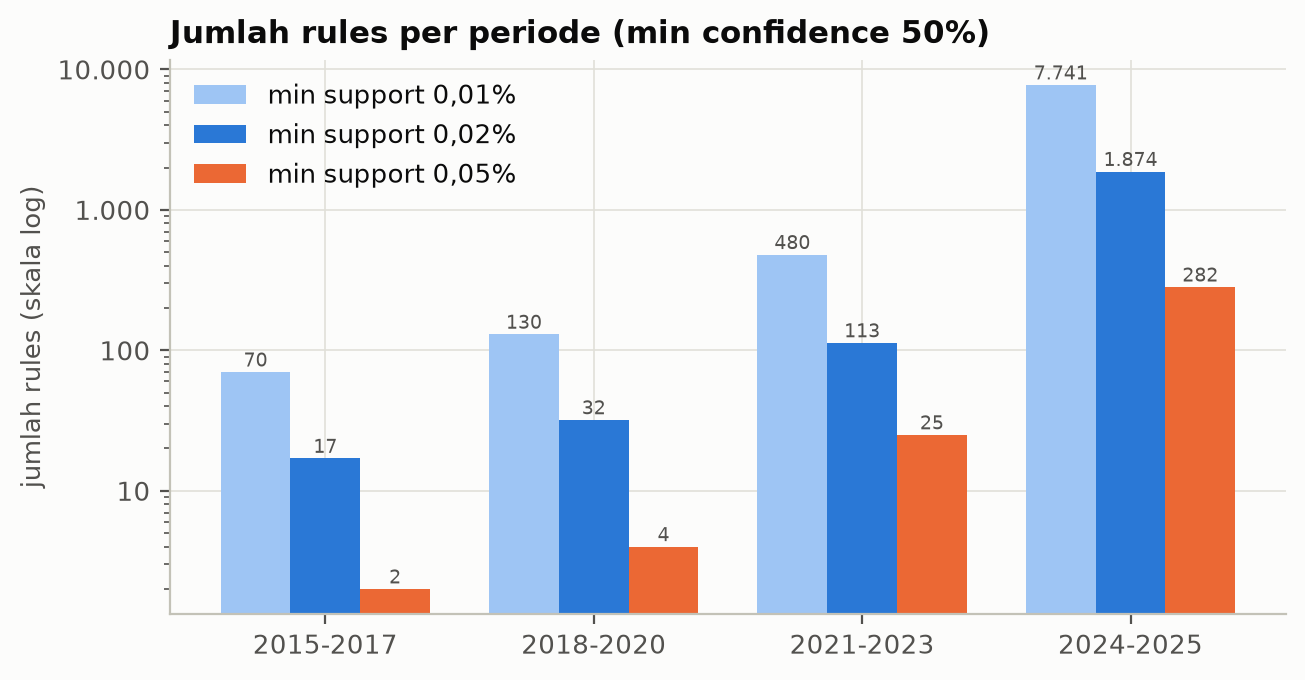
\includegraphics[width=0.9\textwidth]{images/hasil/t7_rules_per_periode.png}
\caption{Jumlah \textit{rules} per periode pada tiga \textit{min\_sup} (skala log, \textit{min\_conf} 50\%)}
\label{fig:e-rules}
\end{figure}

Sepuluh \textit{lift} tertinggi 2015--2017 tersebar di banyak kelompok, misalnya AISTATS + ICML $\Rightarrow$ NeurIPS (\textit{lift} 113,8), ASRU + ICASSP $\Rightarrow$ INTERSPEECH (104,9), dan ACC + ECC $\Rightarrow$ CDC (68,0). Pada 2024--2025, seluruh sepuluh \textit{lift} tertinggi adalah \textit{rule} tiga atau empat konferensi menuju dua konferensi yang memuat ACL atau EMNLP bersama ICLR atau ICML, misalnya EMNLP + ICLR + ACM Multimedia + NeurIPS $\Rightarrow$ ACL + ICML (\textit{lift} 161,9). \textit{Count}-nya hanya 184 sampai 279 transaksi, dan hanya empat dari sepuluh yang lolos uji ketahanan.

\section{Perbandingan \textit{rules} antarperiode}
\label{sec:hasil-e-banding}
Setiap \textit{rule} pada 0,02\% diberi kategori menurut kemunculannya: \textit{bertahan} (lolos di keempat periode), \textit{muncul} (tidak lolos di awal, lalu lolos terus sampai 2024--2025), \textit{hilang} (lolos di awal, lalu tidak lolos sampai 2024--2025), dan \textit{berselang} (pola lain). \textit{Support}, \textit{confidence}, dan \textit{lift} setiap \textit{rule} juga dihitung langsung dari transaksi di setiap periode, termasuk periode saat \textit{rule} itu tidak lolos.

\begin{table}[ht]
\caption{Jumlah \textit{rules} per kategori pada tiga \textit{min\_sup}}
\label{tab:e-kategori}
\small
\begin{tabular}{@{}lrrr@{}}
\toprule
\textbf{Kategori} & \textbf{0,01\%} & \textbf{0,02\% (utama)} & \textbf{0,05\%} \\
\midrule
Bertahan & 13 & 1 & 0 \\
Hilang & 39 & 11 & 2 \\
Berselang & 113 & 27 & 7 \\
Muncul & 7.704 & 1.865 & 281 \\
\bottomrule
\end{tabular}
\end{table}

Tabel~\ref{tab:e-kategori} menunjukkan gambaran yang sama pada ketiga ambang: 97\% sampai 98\% \textit{rules} adalah \textit{rules} yang muncul, dan \textit{rules} yang bertahan sangat sedikit. Jumlah pasti \textit{rules} bertahan bergantung pada ambang (13, 1, dan 0), sehingga yang disimpulkan adalah polanya, bukan angkanya.

\textbf{\textit{Rule} yang bertahan.} Pada 0,02\%, satu-satunya \textit{rule} yang bertahan adalah AISTATS + ICML $\Rightarrow$ NeurIPS. \textit{Confidence}-nya hampir tetap (60\%, 61\%, 61\%, dan 58\%), sedangkan \textit{count}-nya naik dari 204 menjadi 716 pada 2021--2023.

\textbf{\textit{Rules} yang hilang.} Sebelas \textit{rules} hilang, tujuh di antaranya melibatkan GLOBECOM dan ICC. Tabel~\ref{tab:e-hilang} menunjukkan bahwa hilangnya bukan karena hubungan berhenti. Ada tiga penyebab:
\begin{enumerate}
\item \textbf{Data tidak tercatat.} DBLP tidak mencatat ICCC pada 2024--2025, sehingga dua \textit{rule} ICCC hilang karena data. ECOC juga tidak tercatat pada 2016, 2019, dan 2022--2024, dan ICTON tidak tercatat pada 2021--2022.
\item \textbf{\textit{Count} tetap, \textit{database} bertambah.} \textit{Count} \textit{rules} GLOBECOM/ICC relatif datar, sedangkan ambang \textit{count} naik dari 185 menjadi 240 pada 2021--2023 karena jumlah transaksi bertambah. Kombinasinya tidak menghilang, tetapi porsinya mengecil.
\item \textbf{\textit{Confidence} di sekitar 50\%.} Setelah tidak lolos, \textit{confidence} \textit{rules} ini tetap 40\% sampai 64\%, sehingga lolos atau tidaknya ditentukan selisih kecil.
\end{enumerate}
Hanya ACC + ECC $\Rightarrow$ CDC yang \textit{count}-nya juga turun secara absolut (dari 259 menjadi 140).

\begin{table}[ht]
\caption{Beberapa \textit{rule} yang hilang (\textit{min\_sup} 0,02\%; ambang \textit{count} 185, 217, 240, 178)}
\label{tab:e-hilang}
\footnotesize
\setlength{\tabcolsep}{4pt}
\begin{tabular}{@{}lll@{}}
\toprule
\textbf{\textit{Rule}} & \textbf{\textit{Count} per periode} & \textbf{\textit{Confidence} per periode} \\
\midrule
ICC + ICCC $\Rightarrow$ GLOBECOM & 210 / 256 / 325 / 0 & 56\% / 58\% / 59\% / -- \\
GLOBECOM + WCNC $\Rightarrow$ ICC & 475 / 521 / 496 / 533 & 52\% / 48\% / 50\% / 46\% \\
GLOBECOM + SPAWC $\Rightarrow$ ICC & 236 / 194 / 203 / 158 & 63\% / 49\% / 59\% / 54\% \\
ECOC $\Rightarrow$ OFC & 1.721 / 1.558 / 600 / 1.180 & 52\% / 47\% / 48\% / 44\% \\
ASRU $\Rightarrow$ INTERSPEECH & 363 / 221 / 619 / 409 & 50\% / 44\% / 44\% / 47\% \\
ACC + ECC $\Rightarrow$ CDC & 259 / 276 / 170 / 140 & 56\% / 54\% / 49\% / 51\% \\
\bottomrule
\end{tabular}
\end{table}

\textbf{\textit{Rules} yang berselang.} Sebanyak 15 dari 27 \textit{rules} berselang memuat konferensi yang tidak tercatat setiap tahun. Pada DBLP, ICCV hanya tercatat pada tahun ganjil dan ECCV pada tahun genap, sehingga 2015--2017 dan 2021--2023 memiliki dua edisi ICCV, sedangkan 2018--2020 memiliki dua edisi ECCV. Keenam \textit{rule} ICCV hanya lolos pada 2021--2023, dan tiga \textit{rule} ACCV/BMVC dengan ECCV hanya lolos pada 2018--2020. SLT, Odyssey, dan COLING menunjukkan pola yang sama. Pada \textit{author-year-based database}, konferensi seperti ini hanya dapat berpasangan pada tahun penyelenggaraannya, sehingga perbedaan antarperiode untuk konferensi ini terutama mencerminkan jadwal, bukan perubahan minat penulis. Dua belas \textit{rules} sisanya memiliki edisi lengkap di setiap periode dan berselang karena \textit{support} atau \textit{confidence}-nya berada di sekitar ambang.

\textbf{\textit{Rules} yang muncul.} NeurIPS terlibat pada 67\% dari 1.865 \textit{rules} yang muncul, diikuti ICLR (47\%), ACL (45\%), AAAI (43\%), EMNLP (42\%), ICML (40\%), dan CVPR (35\%). Sebanyak 95 \textit{rules} sudah muncul sejak 2018--2020 atau 2021--2023 dan bertahan sampai 2024--2025, dan 94\% sampai 95\% di antaranya lolos uji ketahanan. Sisanya, 1.770 \textit{rules}, hanya ada pada 2024--2025, dan hanya 65\% yang lolos uji ketahanan.

\section{Jawaban pertanyaan Bagian E}
\label{sec:jawab-e}
\textbf{\textit{Frequent itemsets} dan \textit{rules} per periode.} FP-Growth dijalankan pada empat periode dan tiga \textit{min\_sup}. Pada \textit{min\_sup} utama 0,02\%, \textit{itemset} berisi dua konferensi atau lebih berjumlah 279, 376, 662, dan 2.380, dan \textit{rules} berjumlah 17, 32, 113, dan 1.874.

\textbf{Perbandingan dan pola yang bertahan atau berubah.} Hampir seluruh \textit{rules} (98\%) adalah \textit{rules} baru, dan hanya AISTATS + ICML $\Rightarrow$ NeurIPS yang bertahan di keempat periode. \textit{Rules} yang hilang, terutama GLOBECOM/ICC, sebagian besar hanya turun sedikit di bawah ambang karena \textit{count}-nya tetap saat \textit{database} bertambah, atau hilang karena konferensinya tidak tercatat. Lebih dari separuh \textit{rules} yang berselang mengikuti jadwal konferensi yang tidak tahunan.

\textbf{Kemungkinan perubahan tren publikasi.} Pertama, kombinasi konferensi dalam satu tahun makin terpusat pada NeurIPS, ICLR, ICML, ACL, EMNLP, AAAI, dan CVPR. Ini sejalan dengan Subbab~\ref{sec:hasil-tren}, tempat konferensi yang sama tumbuh paling cepat dan porsi sepuluh konferensi teratas naik dari 7,0\% menjadi 11,7\%. Kedua, penulis di konferensi-konferensi ini makin sering menerbitkan di beberapa konferensi besar pada tahun yang sama, termasuk lintas NLP dan \textit{machine learning}. Rata-rata konferensi per transaksi hanya naik dari 1,57 menjadi 1,68, sehingga perubahan ini terkonsentrasi pada konferensi tersebut, bukan pada seluruh penulis. Ketiga, kombinasi di telekomunikasi, kendali, dan komunikasi optik relatif tetap secara absolut tetapi mengecil secara relatif. Tren yang paling dapat dipercaya adalah 95 \textit{rules} yang muncul pada 2018--2023. \textit{Rules} yang hanya ada pada 2024--2025 sebagian dipengaruhi transaksi berisi banyak konferensi dan data 2025 yang belum lengkap.

\chapter{ANALISIS DAN INTERPRETASI}
\label{chap:analisis}

Bab ini merangkum makna temuan seluruh \textit{task}. Angka rinci ada pada bab yang dirujuk.

\section{Makna Hasil Pemahaman Data dan Popularitas}
\begin{enumerate}
\item \textit{Venue} adalah seri yang batasnya ditentukan \textit{key}, sehingga \textit{workshop} yang berbagi \textit{key} ikut konferensi induk (7,2\% makalah). Peringkat berlaku untuk definisi ini, dan NeurIPS tetap nomor satu pada definisi lain (Bab~\ref{chap:popularitas}).
\item Data bersih secara struktural, tetapi identitas penulis tidak pasti: nama umum yang menggabungkan banyak orang (\textit{Yang Liu} pada 332 \textit{venue}) menjadi risiko utama pada seluruh hasil \textit{mining}.
\item Aktivitas sangat terkonsentrasi: separuh publikasi berasal dari 5,3\% \textit{venue}, dan 8,3\% penulis menyumbang 52,6\% pasangan makalah-penulis. Porsi sepuluh konferensi teratas naik dari 7,0\% menjadi 11,7\%, karena konferensi kecerdasan buatan dan pemrosesan bahasa alami tumbuh 3,6 sampai 10,2 kali sedangkan konferensi komunikasi dan biomedis menurun. Data tidak memuat penyebabnya.
\end{enumerate}

\section{Makna Pilihan Representasi Transaksi}
\textit{Author-based} menangkap riwayat penulis selama sebelas tahun, sedangkan \textit{author-year-based} hanya menangkap kemunculan pada tahun yang sama. Akibatnya \textit{support} pasangan pada \textit{author-year-based} median 0,29 kali, sekitar 23\% pasangan tidak pernah muncul, dan konferensi dua tahunan berselang seperti ICCV dan ECCV tidak dapat berpasangan. Pilihan representasi karena itu menentukan pola yang dapat ditemukan (Bab~\ref{chap:transaksi}).

\section{Makna Hasil \textit{Mining}}
\begin{enumerate}
\item \textbf{Keterkaitan konferensi mengelompok per bidang.} Kombinasi teratas adalah ICML dan NeurIPS, dan \textit{itemset} terpanjang berisi enam konferensi kecerdasan buatan dan \textit{computer vision} (Bab~\ref{chap:fpm}). Popularitas tidak sama dengan keterkaitan: NeurIPS memiliki \textit{rules} terbanyak, tetapi \textit{lift} \textit{rules} yang menuju kepadanya rendah karena \textit{lift} dibagi \textit{support} konferensi tujuan. Hubungan satu-ke-satu terkuat justru dimiliki pasangan yang lebih kecil dalam satu bidang, misalnya ECOC dan OFC (Bab~\ref{chap:rules}).
\item \textbf{Performa kedua algoritma setara pada data ini.} Transaksi DBLP pendek dan polanya dangkal, sehingga keunggulan FP-Growth yang tidak membangkitkan kandidat belum terlihat pada waktu, tetapi terlihat pada jumlah kandidat Apriori yang tumbuh kuadratik (Bab~\ref{chap:performa}).
\item \textbf{Perhatian bergeser ke kecerdasan buatan.} Kelompok konferensi yang ditemukan tetap sama antarperiode, tetapi pusatnya bergeser dari GLOBECOM dan ICC ke ICLR dan NeurIPS. Sebagian perubahan ditentukan oleh data, yaitu konferensi yang tidak diadakan setiap tahun dan tahun yang tidak tercatat di DBLP (Bab~\ref{chap:temporal}).
\end{enumerate}

\section{Penafsiran yang Perlu Hati-hati}
\begin{enumerate}
\item Nama penulis umum memengaruhi sebagian \textit{itemset} dan \textit{rules} besar, sehingga hasil dibaca bersama keterbatasan pada Bab~\ref{chap:kesimpulan}.
\item \textit{Lift} dipakai untuk membandingkan \textit{rules}, bukan sebagai ukuran mutlak, karena \textit{min\_conf} 50\% dan \textit{support} konferensi yang rendah menjadikan \textit{lift} minimum cukup tinggi.
\item Data 2025 tidak lengkap sehingga periode 2024--2025 pada Bagian E bias.
\end{enumerate}

\chapter{KESIMPULAN}
\label{chap:kesimpulan}

\section{Jawaban Pertanyaan Kesimpulan}
Pertanyaan kesimpulan pada spesifikasi tugas didasarkan pada seluruh eksperimen. Seluruh \textit{Task} 1 sampai 6 dan Bagian E sudah dikerjakan sehingga ketujuh pertanyaan dapat dijawab.

\begin{enumerate}
\item \textbf{Konferensi dengan popularitas publikasi tertinggi.} NeurIPS, dengan 25.455 makalah (1,27\% dari 1.997.244 publikasi pada 2015--2025) dan 57.800 penulis unik. NeurIPS tetap berada di peringkat pertama ketika \textit{workshop} dan acara satelit dikeluarkan dari perhitungan. Peringkat berikutnya, yaitu CVPR dan ICASSP, bergantung pada definisi: CVPR turun ke peringkat enam jika \textit{CVPR Workshops} dikeluarkan.
\item \textbf{Asosiasi konferensi paling populer dengan konferensi lain.} NeurIPS memiliki asosiasi paling banyak, tetapi bukan yang paling kuat. NeurIPS termasuk dalam 42 pasangan \textit{frequent}, 35 dari 40 \textit{itemset} berisi lima atau enam konferensi, dan menjadi tujuan 240 \textit{rules}, terbanyak dari semua konferensi. Namun, median \textit{lift} \textit{rules} yang menuju NeurIPS hanya 23,61, kedua terendah. Semakin populer sebuah konferensi, semakin rendah \textit{lift} \textit{rules} yang menuju kepadanya (Spearman $-0{,}933$), karena \textit{lift} dibagi dengan \textit{support} konferensi tujuan. Asosiasi satu-ke-satu terkuat justru dimiliki pasangan yang lebih kecil, yaitu ECOC $\Rightarrow$ OFC (\textit{lift} 80,12) dan ASRU $\Rightarrow$ INTERSPEECH (74,17) (Subbab~\ref{sec:hasil-t5-lift}).
\item \textbf{Kombinasi konferensi yang paling sering muncul bersama.} ICML dan NeurIPS (18.503 penulis, \textit{support} 1,02\%), satu-satunya pasangan yang masih \textit{frequent} pada \textit{min\_sup} 1\%, disusul ICLR dan NeurIPS (17.852) serta AAAI dan NeurIPS (15.973). \textit{Triple} teratas adalah ICLR, ICML, dan NeurIPS (10.413 penulis), dan \textit{itemset} terpanjang berisi enam konferensi, yaitu AAAI, CVPR, ECCV, ICCV, ICLR, dan NeurIPS (2.005 penulis) (Subbab~\ref{sec:hasil-t4-fp-kombinasi}).
\item \textbf{\textit{Rule} dengan \textit{lift} tertinggi.} ECCV + ACM Multimedia + NeurIPS $\Rightarrow$ AAAI + CVPR + ICCV (\textit{lift} 172,27). Dari 2.983 penulis yang menerbitkan di ECCV, ACM Multimedia, dan NeurIPS, 61,2\% juga menerbitkan di AAAI, CVPR, dan ICCV, atau 172 kali lebih sering dibanding penulis pada umumnya. \textit{Rule} ini hanya didukung 1.827 penulis, sedikit di atas ambang 1.822, dan tidak lagi lolos jika profil nama umum yang menggabungkan banyak orang dikeluarkan sehingga perlu dibaca hati-hati. \textit{Lift} tingginya terutama berasal dari \textit{consequent} tiga konferensi yang jarang muncul bersama. Di antara \textit{rule} satu-ke-satu, \textit{lift} tertinggi dimiliki ECOC $\Rightarrow$ OFC (80,12): 66,5\% penulis ECOC juga menerbitkan di OFC (Subbab~\ref{sec:hasil-t5-top10} dan \ref{sec:hasil-t5-menarik}).
\item \textbf{Perbedaan pola pada \textit{author-based} dan \textit{author-year-based}.} Ya. Kedua representasi menjawab pertanyaan yang berbeda. \textit{Author-based} menangkap riwayat publikasi selama 2015--2025, sedangkan \textit{author-year-based} hanya menangkap konferensi pada tahun yang sama. Akibatnya, \textit{support} pasangan pada \textit{author-year-based} median 0,29 kali \textit{author-based}, dan ICCV dan ECCV tidak pernah berpasangan (10.051 transaksi pada \textit{author-based}, nol pada \textit{author-year-based}) karena keduanya tercatat pada tahun yang berbeda. Pada \textit{min\_sup} 0,1\%, \textit{author-based} menghasilkan 1.387 \textit{rules}, sedangkan setiap periode \textit{author-year-based} hanya 0 sampai 60, sehingga Bagian E memakai \textit{min\_sup} 0,01\% sampai 0,05\%. Kelompok konferensi yang ditemukan tetap sama (NeurIPS--ICML--ICLR, ACL--EMNLP, CVPR--ICCV/ECCV, GLOBECOM--ICC), dan urutan pasangan teratas relatif terjaga (18 dari 20 sama, korelasi peringkat 0,892). Kelebihan \textit{author-year-based} adalah dimensi waktunya: \textit{database} ini memperlihatkan bahwa 98\% \textit{rules} pada \textit{min\_sup} 0,02\% baru muncul pada periode akhir (Subbab~\ref{sec:hasil-e-banding}).
\item \textbf{Algoritma dengan performa terbaik.} Pada keempat \textit{min\_sup} yang diuji, Apriori dan FP-Growth setara. Keduanya menghasilkan \textit{itemset} dan \textit{rules} yang identik, dan selisih median waktunya paling besar 6\% (5,41 dan 5,19 detik pada 0,1\%), lebih kecil daripada variasi antarpengulangan. Waktu keduanya setara karena transaksi DBLP pendek dan polanya dangkal. FP-Growth tetap dipilih sebagai algoritma utama karena tidak membangkitkan kandidat. Kandidat Apriori tumbuh kuadratik terhadap jumlah item \textit{frequent}: pada 0,1\% terdapat 164.451 pasangan kandidat, dan hanya 0,24\% yang \textit{frequent} (Subbab~\ref{sec:jawab-t6}).
\item \textbf{Pengetahuan atau \textit{insight} utama.} Popularitas dan asosiasi konferensi makin terpusat pada konferensi kecerdasan buatan. Porsi sepuluh konferensi teratas naik dari 7,0\% pada 2015 menjadi 11,7\% pada 2024, dan NeurIPS tumbuh 10,2 kali. Pola asosiasinya mengikuti: pasangan teratas bergeser dari GLOBECOM + ICC pada 2015--2017 ke ICLR + NeurIPS pada 2024--2025, NeurIPS terlibat pada 67\% \textit{rules} yang baru muncul, dan \textit{itemset} berisi empat konferensi atau lebih dalam satu tahun naik dari 1 menjadi 710 (\textit{min\_sup} 0,02\%). Hubungan terkuat tetap berada di dalam satu bidang dan mengarah dari konferensi kecil ke konferensi besar, sedangkan konferensi terpopuler justru memiliki \textit{lift} rendah. Kombinasi di bidang lain, misalnya GLOBECOM dan ICC, tidak menghilang tetapi porsinya mengecil. Terakhir, sebagian pola ditentukan oleh data, bukan oleh perilaku penulis: nama umum yang menggabungkan banyak orang, konferensi yang tidak diadakan setiap tahun, dan tahun yang tidak tercatat di DBLP (Subbab~\ref{sec:jawab-e}).
\end{enumerate}

\section{Keterbatasan dan Asumsi}
\begin{enumerate}
\item \textit{Venue} diambil dari segmen kedua \textit{key} sehingga \textit{workshop} dan acara pendamping ikut terhitung sebagai konferensi induknya (7,2\% makalah menurut \textit{booktitle}). Dampaknya besar pada CVPR, CHI, dan ICC (Tabel~\ref{tab:sensitivitas}).
\item \textit{Record} \texttt{inproceedings} yang \textit{key}-nya bukan \texttt{conf/} (3.161 makalah, 0,16\%) dibuang, termasuk beberapa prosiding \textit{workshop} kecil.
\item Data 2025 tidak lengkap karena konferensi dua tahunan genap dan konferensi tahunan yang belum terindeks sehingga tidak dipakai menghitung tren dan membuat transaksi \textit{author-year-based} pada periode terakhir bias.
\item Nama penulis umum tanpa sufiks disambiguasi dapat mewakili banyak orang (\textit{Yang Liu} tercatat pada 332 \textit{venue}), dan 7.573 kelompok nama yang hanya berbeda diakritik atau huruf besar-kecil tidak digabung. Akibatnya, penulis unik cenderung terhitung lebih rendah dan sebagian transaksi menjadi terlalu besar.
\item Aturan duplikat berdasarkan judul, tahun, dan \textit{venue} dapat membuang sebagian makalah berbeda yang berjudul generik (paling banyak 421 baris, 0,02\% data).
\item ICLR tidak tercatat pada DBLP untuk 2015 dan 2016 sehingga dikeluarkan dari \textit{heatmap} indeks.
\item Pengenalan acara satelit lewat kata kunci \textit{booktitle} adalah pendekatan. Beberapa acara resmi, misalnya \textit{CHI Extended Abstracts}, dapat dianggap bagian konferensi utama.
\item Model transaksi berupa himpunan tidak menyimpan jumlah makalah per \textit{venue}: 38,3\% makalah pada \textit{author-based} dan 17,4\% pada \textit{author-year-based} tidak menambah item baru (Subbab~\ref{sec:hasil-npaper}).
\item Pratinjau perbandingan pasangan hanya mencakup \textit{venue} dengan \textit{support} minimal 0,1\% pada \textit{author-based} (574 \textit{venue}) dan belum merupakan hasil \textit{mining}.
\item Popularitas hanya diukur dari aktivitas publikasi, bukan dari sitasi atau kualitas. Pengelompokan bidang konferensi pada narasi adalah pengetahuan umum, bukan atribut dari data DBLP. Pada Bab~\ref{sec:hasil-t4} dan \ref{sec:hasil-t5}, nama bidang dicocokkan dengan judul prosiding pada data DBLP.
\item Pada \textit{min\_sup} 0,1\%, 291 transaksi dengan 100 konferensi atau lebih, yang hampir seluruhnya nama umum tanpa nomor disambiguasi, menentukan lolos tidaknya sebagian \textit{itemset}. Tanpa transaksi tersebut, 109 dari 1.514 \textit{frequent itemsets} (7\%) dan tujuh dari sepuluh \textit{rule} dengan \textit{lift} tertinggi tidak lagi lolos ambang. Hasil tetap dilaporkan apa adanya.
\item Dengan \textit{min\_conf} 50\% dan \textit{support} setiap konferensi di bawah 3,2\%, setiap \textit{rule} otomatis memiliki \textit{lift} minimal sekitar 15,8. \textit{Lift} pada data ini dipakai untuk membandingkan \textit{rules}, bukan sebagai ukuran mutlak.
\item \textit{Rules} hanya ada untuk kombinasi yang lolos \textit{min\_sup}. Hubungan kuat antara dua konferensi kecil tidak terlihat.
\item Pada Bagian E, konferensi yang tidak tercatat setiap tahun (misalnya ICCV, ECCV, ASRU, SLT) dan tahun yang tidak tercatat di DBLP (misalnya ICCC pada 2024--2025) membuat sebagian \textit{rules} muncul atau hilang karena data. Hanya 67\% \textit{rules} 2024--2025 pada \textit{min\_sup} 0,02\% yang tetap ditemukan tanpa transaksi berisi 20 konferensi atau lebih, sehingga kriteria ketahanan 80\% tidak terpenuhi pada periode ini.
\item Perbandingan waktu pada \textit{Task} 6 memakai implementasi Python murni satu \textit{thread} dengan tiga pengulangan pada satu komputer. Waktu absolutnya dapat berbeda pada implementasi lain, dan selisih median beberapa persen tidak dianggap bermakna.
\end{enumerate}


\cleardoublepage
\printbibliography[heading=bibintoc, title={DAFTAR PUSTAKA}]

\appendix
\begin{appendices}
\addtocontents{toc}{\protect\renewcommand{\protect\cftchappresnum}{}}
\addtocontents{toc}{\protect\settowidth{\protect\cftchapnumwidth}{A\quad}}
\chapter{Pembagian Kerja}
\lampirancaption{Pembagian Kerja}
\label{lamp:pembagian}

\begin{table}[ht]
\caption{Pembagian kerja anggota kelompok}
\label{tab:pembagian}
\small
\begin{tabularx}{\textwidth}{@{}>{\raggedright\arraybackslash}p{4.2cm}>{\raggedright\arraybackslash}X@{}}
\toprule
\textbf{Anggota} & \textbf{Pekerjaan} \\
\midrule
Izhar Alif Akbar (18223129) & \textit{Task} 1 sampai \textit{Task} 3, membantu analisis \textit{Task} 6, dan kesimpulan \\
\midrule
Harfhan Ikhtiar (18223123) & Implementasi Apriori pada \textit{Task} 4 dan \textit{Task} 5, dan \textit{Task} 6 bersama \\
\midrule
Mahesa Andre (13523140) & Implementasi FP-Growth pada \textit{Task} 4 dan \textit{Task} 5, dan \textit{Task} 6 bersama \\
\midrule
Bersama & Analisis \textit{Task} 6 dan kesimpulan \\
\bottomrule
\end{tabularx}
\end{table}

\chapter{Hasil \textit{Transactional Database}}
\lampirancaption{Hasil \textit{Transactional Database}}
\label{lamp:transaksi}

Lampiran ini memperlihatkan isi berkas hasil \textit{Task} 3 dan beberapa instance nyata dari data. Seluruh isi diambil langsung dari berkas pada folder \texttt{data/processed/}.

\section{Berkas hasil}
Tabel~\ref{tab:berkas-tx} merangkum lima berkas hasil. Tabel panjang menyimpan pasangan \texttt{(tid, item)} satu baris per pasangan. Tabel indeks memetakan \texttt{tid} ke identitas transaksi, dan \texttt{item} berupa kode integer yang dipetakan ke nama \textit{venue} oleh \texttt{tx\_items.csv}.

\begin{table}[ht]
\caption{Berkas hasil pembentukan \textit{transactional database}}
\label{tab:berkas-tx}
\scriptsize
\begin{tabularx}{\textwidth}{@{}p{5.0cm}>{\raggedright\arraybackslash}Xrr@{}}
\toprule
\textbf{Berkas} & \textbf{Kolom (tipe)} & \textbf{Baris} & \textbf{Ukuran} \\
\midrule
\texttt{tx\_items.csv} & \texttt{venue}, \texttt{item\_id}, \texttt{nama} & 4.373 & 0,08 MB \\
\texttt{tx\_author.parquet} & \texttt{tid} (int32), \texttt{item} (int32) & 4.853.675 & 20 MB \\
\texttt{tx\_author\_index.parquet} & \texttt{tid}, \texttt{author} (string), \texttt{n\_paper} (int32) & 1.821.757 & 36 MB \\
\texttt{tx\_author\_year.parquet} & \texttt{tid} (int32), \texttt{item} (int32) & 6.497.515 & 31 MB \\
\texttt{tx\_author\_year\_index.parquet} & \texttt{tid}, \texttt{author}, \texttt{year} (int16), \texttt{n\_paper} & 4.085.594 & 75 MB \\
\bottomrule
\end{tabularx}
\end{table}

\section{Cuplikan berkas}
Tabel~\ref{tab:cuplikan-items} sampai Tabel~\ref{tab:cuplikan-index} menampilkan baris pertama dari tiap berkas, dan item pada Tabel~\ref{tab:cuplikan-a} dapat dicocokkan dengan \texttt{tid} yang sama pada Tabel~\ref{tab:cuplikan-a-index}.

\begin{table}[ht]
\caption{Lima baris pertama \texttt{tx\_items.csv}}
\label{tab:cuplikan-items}
\small
\begin{tabular}{@{}lp{7.2cm}r@{}}
\toprule
\textbf{\texttt{venue}} (segmen \textit{key}) & \textbf{\texttt{nama}} & \textbf{\texttt{item\_id}} \\
\midrule
\texttt{3dic} & 3DIC & 0 \\
\texttt{3dica} & \textit{3D Image Processing, Measurement (3DIPM), and Applications} & 1 \\
\texttt{3dim} & 3DV & 2 \\
\texttt{3dor} & 3DOR@Eurographics & 3 \\
\texttt{3dtv} & 3DTV-Conference & 4 \\
\bottomrule
\end{tabular}
\end{table}

\begin{table}[ht]
\caption{Cuplikan \texttt{tx\_author.parquet} (tabel panjang \textit{author-based}, \texttt{tid} 0 dan 1)}
\label{tab:cuplikan-a}
\small
\begin{tabular}{@{}rrl@{}}
\toprule
\textbf{\texttt{tid}} & \textbf{\texttt{item}} & \textbf{Nama \textit{venue}} \\
\midrule
0 & 1007 & DAC \\
1 & 1007 & DAC \\
1 & 1161 & DSN \\
1 & 1375 & ETS \\
1 & 1737 & HPCA \\
1 & 2486 & IOLTS \\
1 & \multicolumn{1}{c}{\ldots} & \multicolumn{1}{c}{\ldots} \\
\bottomrule
\end{tabular}
\end{table}

\begin{table}[ht]
\caption{Cuplikan \texttt{tx\_author\_index.parquet} (tabel indeks \textit{author-based}, \texttt{tid} 0 dan 1)}
\label{tab:cuplikan-a-index}
\small
\begin{tabular}{@{}rlr@{}}
\toprule
\textbf{\texttt{tid}} & \textbf{\texttt{author}} & \textbf{\texttt{n\_paper}} \\
\midrule
0 & Lucas Roquet & 1 \\
1 & Fernando Fernandes dos Santos & 24 \\
\bottomrule
\end{tabular}
\end{table}

\begin{table}[ht]
\caption{Cuplikan tabel indeks \textit{author-year-based} (\texttt{tid} 0 sampai 5)}
\label{tab:cuplikan-index}
\small
\begin{tabular}{@{}rlrr@{}}
\toprule
\textbf{\texttt{tid}} & \textbf{\texttt{author}} & \textbf{\texttt{year}} & \textbf{\texttt{n\_paper}} \\
\midrule
0 & Lucas Roquet & 2024 & 1 \\
1 & Fernando Fernandes dos Santos & 2024 & 5 \\
2 & Paolo Rech & 2024 & 5 \\
3 & Marcello Traiola & 2024 & 8 \\
4 & Olivier Sentieys & 2024 & 8 \\
5 & Angeliki Kritikakou & 2024 & 9 \\
\bottomrule
\end{tabular}
\end{table}

\section{\textit{Instance} nyata 1: penulis dengan 10 makalah}
\label{sec:instance1}
Penulis pada Gambar~\ref{fig:ilustrasi} adalah \textit{Brian Camilo Gómez-León} (\texttt{tid} 127307 pada \textit{author-based}). Tabel~\ref{tab:instance-paper} menunjukkan 10 makalahnya pada \texttt{paper\_author.parquet}, dan Tabel~\ref{tab:instance-tx} menunjukkan transaksi yang terbentuk dari makalah-makalah tersebut. Segmen kedua \textit{key} menentukan \textit{venue}, misalnya \texttt{iceee} bernama tampilan CCE dan \texttt{amcc} bernama tampilan ACC.

\begin{table}[ht]
\caption{Sepuluh makalah \textit{Brian Camilo Gómez-León} pada \texttt{paper\_author.parquet}}
\label{tab:instance-paper}
\footnotesize
\begin{tabular}{@{}llrl@{}}
\toprule
\textbf{\textit{Key}} & \textbf{\texttt{venue}} & \textbf{Tahun} & \textbf{Nama tampilan} \\
\midrule
\texttt{conf/ccta/Sira-RamirezGAZ21} & \texttt{ccta} & 2021 & CCTA \\
\texttt{conf/iccad2/Sira-RamirezGA21} & \texttt{iccad2} & 2021 & ICCAD [iccad2] \\
\texttt{conf/iceee/Gomez-LeonAS21} & \texttt{iceee} & 2021 & CCE \\
\texttt{conf/cdc/Aguilar-OrdunaS22} & \texttt{cdc} & 2022 & CDC \\
\texttt{conf/iceee/Aguilar-OrdunaS22} & \texttt{iceee} & 2022 & CCE \\
\texttt{conf/vss/Sira-RamirezAG22} & \texttt{vss} & 2022 & VSS \\
\texttt{conf/iceee/AguilarOrdunaSGG23} & \texttt{iceee} & 2023 & CCE \\
\texttt{conf/iceee/HernandezAGS23} & \texttt{iceee} & 2023 & CCE \\
\texttt{conf/amcc/GomezLeonASG24} & \texttt{amcc} & 2024 & ACC \\
\texttt{conf/amcc/SiraRamirezGA24} & \texttt{amcc} & 2024 & ACC \\
\bottomrule
\end{tabular}
\end{table}

\begin{table}[ht]
\caption{Transaksi yang terbentuk dari 10 makalah pada Tabel~\ref{tab:instance-paper}}
\label{tab:instance-tx}
\footnotesize
\begin{tabularx}{\textwidth}{@{}p{4.4cm}rrX@{}}
\toprule
\textbf{\textit{Database}} & \textbf{\texttt{tid}} & \textbf{Makalah} & \textbf{Isi transaksi} \\
\midrule
\textit{Author-based} & 127307 & 10 & CCTA, ICCAD [iccad2], CCE, CDC, VSS, ACC \\
\midrule
\textit{Author-year-based}, 2021 & 993297 & 3 & CCTA, ICCAD [iccad2], CCE \\
\textit{Author-year-based}, 2022 & 199569 & 3 & CDC, CCE, VSS \\
\textit{Author-year-based}, 2023 & 1565683 & 2 & CCE \\
\textit{Author-year-based}, 2024 & 2668311 & 2 & ACC \\
\bottomrule
\end{tabularx}
\end{table}

\section{\textit{Instance} nyata 2: penulis yang aktif delapan tahun}
\label{sec:instance2}
\textit{Fernando Fernandes dos Santos} menerbitkan 24 makalah pada 2017--2025. Pada \textit{author-based}, ia menjadi satu transaksi (\texttt{tid} 1) berisi 11 item, yaitu DAC, DSN, ETS, HPCA, IOLTS, IPDPS, ISVLSI, ITC, SC, VLSI-SoC, dan VTS. Dalam bentuk horizontal dengan kode integer, transaksi ini berbentuk \texttt{frozenset(\{1007, 1161, 1375, 1737, 2486, 2512, 2659, 2673, 3638, 4171, 4200\})}. Pada \textit{author-year-based}, ia menjadi delapan transaksi (Tabel~\ref{tab:instance2}). Contoh ini menunjukkan bahwa satu penulis aktif menyumbang banyak transaksi pada \textit{author-year-based}, dan bahwa IOLTS serta ETS dihitung berulang sebagai pasangan yang sama pada beberapa tahun.

\begin{table}[ht]
\caption{Delapan transaksi \textit{author-year-based} milik \textit{Fernando Fernandes dos Santos}}
\label{tab:instance2}
\footnotesize
\begin{tabularx}{\textwidth}{@{}rrrX@{}}
\toprule
\textbf{\texttt{tid}} & \textbf{Tahun} & \textbf{Makalah} & \textbf{Isi transaksi} \\
\midrule
2692157 & 2017 & 2 & DSN, SC \\
2100036 & 2019 & 3 & ETS, HPCA, IOLTS \\
3858468 & 2020 & 2 & ETS, IOLTS \\
133786 & 2021 & 4 & DSN, IOLTS, IPDPS, VTS \\
577535 & 2022 & 4 & IOLTS, ISVLSI, ITC \\
2693558 & 2023 & 3 & ETS, ITC, SC \\
1 & 2024 & 5 & DAC, ETS, IOLTS, VLSI-SoC, VTS \\
4043841 & 2025 & 1 & ETS \\
\bottomrule
\end{tabularx}
\end{table}

Jumlah makalah per tahun pada Tabel~\ref{tab:instance2} berjumlah 24 (2+3+2+4+4+3+5+1) dan sesuai dengan kolom \texttt{n\_paper} pada transaksi \textit{author-based}. Pada contoh ini, 24 makalah hanya menghasilkan 11 item pada \textit{author-based}, yang berarti sebagian besar makalah tidak menambah item baru.

\end{appendices}
\backmatter
\end{document}
